% Created by tikzDevice version 0.12.6 on 2025-02-15 08:44:33
% !TEX encoding = UTF-8 Unicode
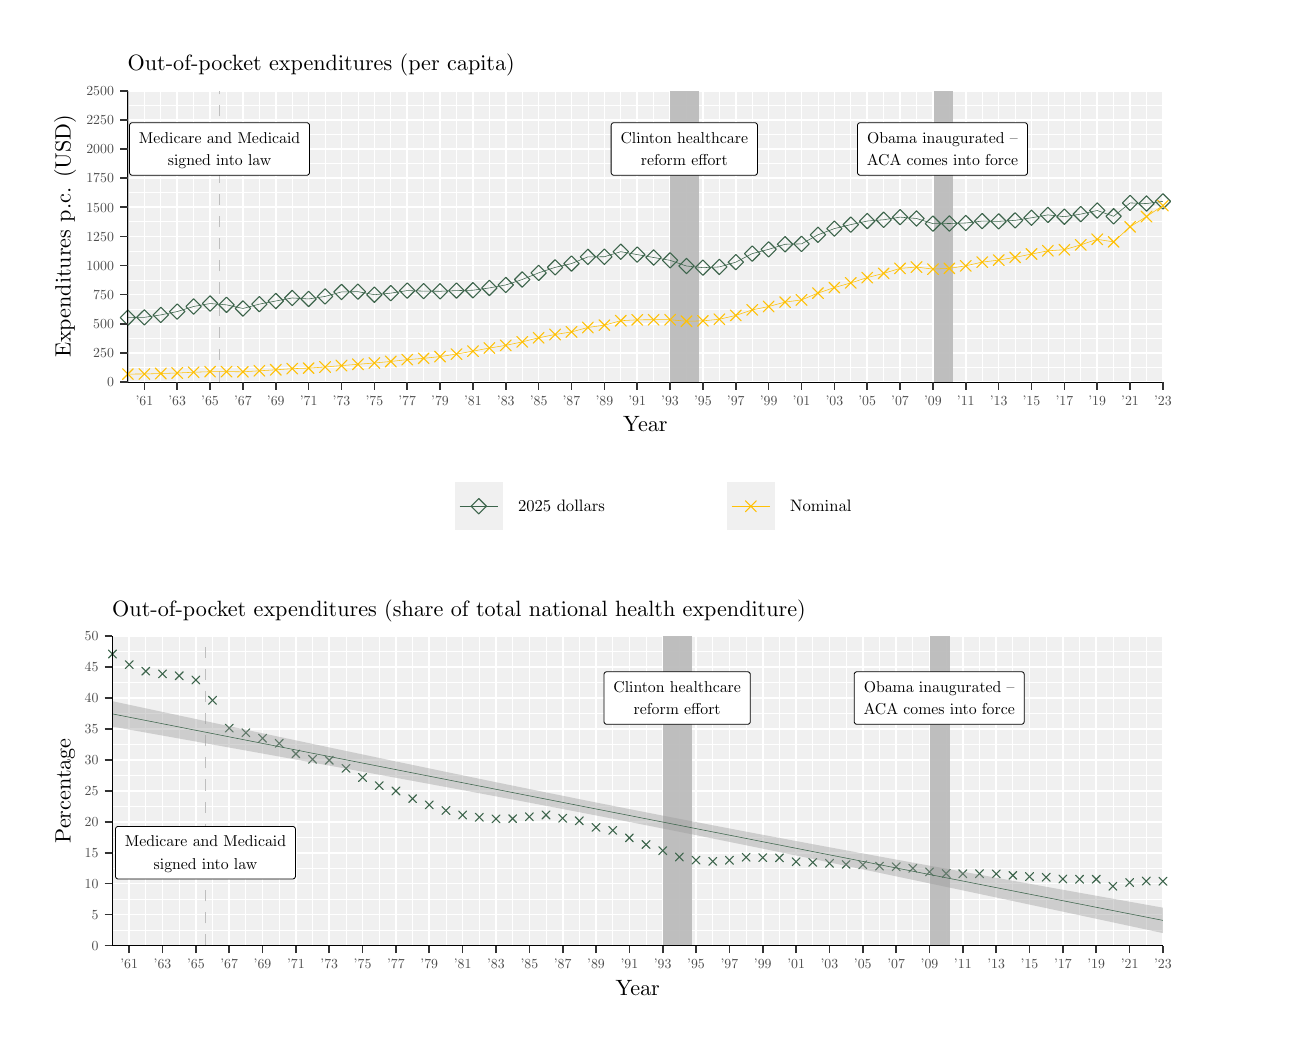
\begin{tikzpicture}[x=1pt,y=1pt]
\definecolor{fillColor}{RGB}{255,255,255}
\path[use as bounding box,fill=fillColor,fill opacity=0.00] (0,0) rectangle (455.30,361.35);
\begin{scope}
\path[clip] (  0.00,164.25) rectangle (455.30,361.35);
\definecolor{drawColor}{RGB}{255,255,255}
\definecolor{fillColor}{RGB}{255,255,255}

\path[draw=drawColor,line width= 0.6pt,line join=round,line cap=round,fill=fillColor] (  0.00,164.25) rectangle (455.30,361.35);
\end{scope}
\begin{scope}
\path[clip] (  0.00,  0.00) rectangle (455.30,361.35);
\definecolor{fillColor}{gray}{0.94}

\path[fill=fillColor] ( 36.14,233.28) rectangle (410.30,338.57);
\definecolor{drawColor}{RGB}{255,255,255}

\path[draw=drawColor,line width= 0.3pt,line join=round] ( 36.14,238.54) --
	(410.30,238.54);

\path[draw=drawColor,line width= 0.3pt,line join=round] ( 36.14,249.07) --
	(410.30,249.07);

\path[draw=drawColor,line width= 0.3pt,line join=round] ( 36.14,259.60) --
	(410.30,259.60);

\path[draw=drawColor,line width= 0.3pt,line join=round] ( 36.14,270.13) --
	(410.30,270.13);

\path[draw=drawColor,line width= 0.3pt,line join=round] ( 36.14,280.66) --
	(410.30,280.66);

\path[draw=drawColor,line width= 0.3pt,line join=round] ( 36.14,291.19) --
	(410.30,291.19);

\path[draw=drawColor,line width= 0.3pt,line join=round] ( 36.14,301.72) --
	(410.30,301.72);

\path[draw=drawColor,line width= 0.3pt,line join=round] ( 36.14,312.25) --
	(410.30,312.25);

\path[draw=drawColor,line width= 0.3pt,line join=round] ( 36.14,322.78) --
	(410.30,322.78);

\path[draw=drawColor,line width= 0.3pt,line join=round] ( 36.14,333.31) --
	(410.30,333.31);

\path[draw=drawColor,line width= 0.3pt,line join=round] ( 36.23,233.28) --
	( 36.23,338.57);

\path[draw=drawColor,line width= 0.3pt,line join=round] ( 48.10,233.28) --
	( 48.10,338.57);

\path[draw=drawColor,line width= 0.3pt,line join=round] ( 59.97,233.28) --
	( 59.97,338.57);

\path[draw=drawColor,line width= 0.3pt,line join=round] ( 71.85,233.28) --
	( 71.85,338.57);

\path[draw=drawColor,line width= 0.3pt,line join=round] ( 83.72,233.28) --
	( 83.72,338.57);

\path[draw=drawColor,line width= 0.3pt,line join=round] ( 95.59,233.28) --
	( 95.59,338.57);

\path[draw=drawColor,line width= 0.3pt,line join=round] (107.46,233.28) --
	(107.46,338.57);

\path[draw=drawColor,line width= 0.3pt,line join=round] (119.34,233.28) --
	(119.34,338.57);

\path[draw=drawColor,line width= 0.3pt,line join=round] (131.21,233.28) --
	(131.21,338.57);

\path[draw=drawColor,line width= 0.3pt,line join=round] (143.08,233.28) --
	(143.08,338.57);

\path[draw=drawColor,line width= 0.3pt,line join=round] (154.96,233.28) --
	(154.96,338.57);

\path[draw=drawColor,line width= 0.3pt,line join=round] (166.83,233.28) --
	(166.83,338.57);

\path[draw=drawColor,line width= 0.3pt,line join=round] (178.70,233.28) --
	(178.70,338.57);

\path[draw=drawColor,line width= 0.3pt,line join=round] (190.58,233.28) --
	(190.58,338.57);

\path[draw=drawColor,line width= 0.3pt,line join=round] (202.45,233.28) --
	(202.45,338.57);

\path[draw=drawColor,line width= 0.3pt,line join=round] (214.32,233.28) --
	(214.32,338.57);

\path[draw=drawColor,line width= 0.3pt,line join=round] (226.19,233.28) --
	(226.19,338.57);

\path[draw=drawColor,line width= 0.3pt,line join=round] (238.07,233.28) --
	(238.07,338.57);

\path[draw=drawColor,line width= 0.3pt,line join=round] (249.94,233.28) --
	(249.94,338.57);

\path[draw=drawColor,line width= 0.3pt,line join=round] (261.81,233.28) --
	(261.81,338.57);

\path[draw=drawColor,line width= 0.3pt,line join=round] (273.69,233.28) --
	(273.69,338.57);

\path[draw=drawColor,line width= 0.3pt,line join=round] (285.56,233.28) --
	(285.56,338.57);

\path[draw=drawColor,line width= 0.3pt,line join=round] (297.43,233.28) --
	(297.43,338.57);

\path[draw=drawColor,line width= 0.3pt,line join=round] (309.30,233.28) --
	(309.30,338.57);

\path[draw=drawColor,line width= 0.3pt,line join=round] (321.18,233.28) --
	(321.18,338.57);

\path[draw=drawColor,line width= 0.3pt,line join=round] (333.05,233.28) --
	(333.05,338.57);

\path[draw=drawColor,line width= 0.3pt,line join=round] (344.92,233.28) --
	(344.92,338.57);

\path[draw=drawColor,line width= 0.3pt,line join=round] (356.80,233.28) --
	(356.80,338.57);

\path[draw=drawColor,line width= 0.3pt,line join=round] (368.67,233.28) --
	(368.67,338.57);

\path[draw=drawColor,line width= 0.3pt,line join=round] (380.54,233.28) --
	(380.54,338.57);

\path[draw=drawColor,line width= 0.3pt,line join=round] (392.41,233.28) --
	(392.41,338.57);

\path[draw=drawColor,line width= 0.3pt,line join=round] (404.29,233.28) --
	(404.29,338.57);

\path[draw=drawColor,line width= 0.6pt,line join=round] ( 36.14,233.28) --
	(410.30,233.28);

\path[draw=drawColor,line width= 0.6pt,line join=round] ( 36.14,243.81) --
	(410.30,243.81);

\path[draw=drawColor,line width= 0.6pt,line join=round] ( 36.14,254.34) --
	(410.30,254.34);

\path[draw=drawColor,line width= 0.6pt,line join=round] ( 36.14,264.87) --
	(410.30,264.87);

\path[draw=drawColor,line width= 0.6pt,line join=round] ( 36.14,275.40) --
	(410.30,275.40);

\path[draw=drawColor,line width= 0.6pt,line join=round] ( 36.14,285.93) --
	(410.30,285.93);

\path[draw=drawColor,line width= 0.6pt,line join=round] ( 36.14,296.46) --
	(410.30,296.46);

\path[draw=drawColor,line width= 0.6pt,line join=round] ( 36.14,306.99) --
	(410.30,306.99);

\path[draw=drawColor,line width= 0.6pt,line join=round] ( 36.14,317.51) --
	(410.30,317.51);

\path[draw=drawColor,line width= 0.6pt,line join=round] ( 36.14,328.04) --
	(410.30,328.04);

\path[draw=drawColor,line width= 0.6pt,line join=round] ( 36.14,338.57) --
	(410.30,338.57);

\path[draw=drawColor,line width= 0.6pt,line join=round] ( 42.17,233.28) --
	( 42.17,338.57);

\path[draw=drawColor,line width= 0.6pt,line join=round] ( 54.03,233.28) --
	( 54.03,338.57);

\path[draw=drawColor,line width= 0.6pt,line join=round] ( 65.91,233.28) --
	( 65.91,338.57);

\path[draw=drawColor,line width= 0.6pt,line join=round] ( 77.78,233.28) --
	( 77.78,338.57);

\path[draw=drawColor,line width= 0.6pt,line join=round] ( 89.66,233.28) --
	( 89.66,338.57);

\path[draw=drawColor,line width= 0.6pt,line join=round] (101.52,233.28) --
	(101.52,338.57);

\path[draw=drawColor,line width= 0.6pt,line join=round] (113.41,233.28) --
	(113.41,338.57);

\path[draw=drawColor,line width= 0.6pt,line join=round] (125.27,233.28) --
	(125.27,338.57);

\path[draw=drawColor,line width= 0.6pt,line join=round] (137.15,233.28) --
	(137.15,338.57);

\path[draw=drawColor,line width= 0.6pt,line join=round] (149.02,233.28) --
	(149.02,338.57);

\path[draw=drawColor,line width= 0.6pt,line join=round] (160.90,233.28) --
	(160.90,338.57);

\path[draw=drawColor,line width= 0.6pt,line join=round] (172.76,233.28) --
	(172.76,338.57);

\path[draw=drawColor,line width= 0.6pt,line join=round] (184.64,233.28) --
	(184.64,338.57);

\path[draw=drawColor,line width= 0.6pt,line join=round] (196.51,233.28) --
	(196.51,338.57);

\path[draw=drawColor,line width= 0.6pt,line join=round] (208.39,233.28) --
	(208.39,338.57);

\path[draw=drawColor,line width= 0.6pt,line join=round] (220.25,233.28) --
	(220.25,338.57);

\path[draw=drawColor,line width= 0.6pt,line join=round] (232.13,233.28) --
	(232.13,338.57);

\path[draw=drawColor,line width= 0.6pt,line join=round] (244.00,233.28) --
	(244.00,338.57);

\path[draw=drawColor,line width= 0.6pt,line join=round] (255.88,233.28) --
	(255.88,338.57);

\path[draw=drawColor,line width= 0.6pt,line join=round] (267.74,233.28) --
	(267.74,338.57);

\path[draw=drawColor,line width= 0.6pt,line join=round] (279.63,233.28) --
	(279.63,338.57);

\path[draw=drawColor,line width= 0.6pt,line join=round] (291.49,233.28) --
	(291.49,338.57);

\path[draw=drawColor,line width= 0.6pt,line join=round] (303.37,233.28) --
	(303.37,338.57);

\path[draw=drawColor,line width= 0.6pt,line join=round] (315.24,233.28) --
	(315.24,338.57);

\path[draw=drawColor,line width= 0.6pt,line join=round] (327.12,233.28) --
	(327.12,338.57);

\path[draw=drawColor,line width= 0.6pt,line join=round] (338.98,233.28) --
	(338.98,338.57);

\path[draw=drawColor,line width= 0.6pt,line join=round] (350.86,233.28) --
	(350.86,338.57);

\path[draw=drawColor,line width= 0.6pt,line join=round] (362.73,233.28) --
	(362.73,338.57);

\path[draw=drawColor,line width= 0.6pt,line join=round] (374.61,233.28) --
	(374.61,338.57);

\path[draw=drawColor,line width= 0.6pt,line join=round] (386.47,233.28) --
	(386.47,338.57);

\path[draw=drawColor,line width= 0.6pt,line join=round] (398.35,233.28) --
	(398.35,338.57);

\path[draw=drawColor,line width= 0.6pt,line join=round] (410.22,233.28) --
	(410.22,338.57);
\definecolor{drawColor}{RGB}{190,190,190}

\path[draw=drawColor,line width= 0.6pt,line join=round] ( 36.22,233.28) -- ( 36.22,338.57);
\definecolor{fillColor}{RGB}{190,190,190}

\path[fill=fillColor,fill opacity=0.01] (232.13,233.28) rectangle (242.42,338.57);

\path[fill=fillColor,fill opacity=0.01] (232.13,233.28) rectangle (242.42,338.57);

\path[fill=fillColor,fill opacity=0.01] (232.13,233.28) rectangle (242.42,338.57);

\path[fill=fillColor,fill opacity=0.01] (232.13,233.28) rectangle (242.42,338.57);

\path[fill=fillColor,fill opacity=0.01] (232.13,233.28) rectangle (242.42,338.57);

\path[fill=fillColor,fill opacity=0.01] (232.13,233.28) rectangle (242.42,338.57);

\path[fill=fillColor,fill opacity=0.01] (232.13,233.28) rectangle (242.42,338.57);

\path[fill=fillColor,fill opacity=0.01] (232.13,233.28) rectangle (242.42,338.57);

\path[fill=fillColor,fill opacity=0.01] (232.13,233.28) rectangle (242.42,338.57);

\path[fill=fillColor,fill opacity=0.01] (232.13,233.28) rectangle (242.42,338.57);

\path[fill=fillColor,fill opacity=0.01] (232.13,233.28) rectangle (242.42,338.57);

\path[fill=fillColor,fill opacity=0.01] (232.13,233.28) rectangle (242.42,338.57);

\path[fill=fillColor,fill opacity=0.01] (232.13,233.28) rectangle (242.42,338.57);

\path[fill=fillColor,fill opacity=0.01] (232.13,233.28) rectangle (242.42,338.57);

\path[fill=fillColor,fill opacity=0.01] (232.13,233.28) rectangle (242.42,338.57);

\path[fill=fillColor,fill opacity=0.01] (232.13,233.28) rectangle (242.42,338.57);

\path[fill=fillColor,fill opacity=0.01] (232.13,233.28) rectangle (242.42,338.57);

\path[fill=fillColor,fill opacity=0.01] (232.13,233.28) rectangle (242.42,338.57);

\path[fill=fillColor,fill opacity=0.01] (232.13,233.28) rectangle (242.42,338.57);

\path[fill=fillColor,fill opacity=0.01] (232.13,233.28) rectangle (242.42,338.57);

\path[fill=fillColor,fill opacity=0.01] (232.13,233.28) rectangle (242.42,338.57);

\path[fill=fillColor,fill opacity=0.01] (232.13,233.28) rectangle (242.42,338.57);

\path[fill=fillColor,fill opacity=0.01] (232.13,233.28) rectangle (242.42,338.57);

\path[fill=fillColor,fill opacity=0.01] (232.13,233.28) rectangle (242.42,338.57);

\path[fill=fillColor,fill opacity=0.01] (232.13,233.28) rectangle (242.42,338.57);

\path[fill=fillColor,fill opacity=0.01] (232.13,233.28) rectangle (242.42,338.57);

\path[fill=fillColor,fill opacity=0.01] (232.13,233.28) rectangle (242.42,338.57);

\path[fill=fillColor,fill opacity=0.01] (232.13,233.28) rectangle (242.42,338.57);

\path[fill=fillColor,fill opacity=0.01] (232.13,233.28) rectangle (242.42,338.57);

\path[fill=fillColor,fill opacity=0.01] (232.13,233.28) rectangle (242.42,338.57);

\path[fill=fillColor,fill opacity=0.01] (232.13,233.28) rectangle (242.42,338.57);

\path[fill=fillColor,fill opacity=0.01] (232.13,233.28) rectangle (242.42,338.57);

\path[fill=fillColor,fill opacity=0.01] (232.13,233.28) rectangle (242.42,338.57);

\path[fill=fillColor,fill opacity=0.01] (232.13,233.28) rectangle (242.42,338.57);

\path[fill=fillColor,fill opacity=0.01] (232.13,233.28) rectangle (242.42,338.57);

\path[fill=fillColor,fill opacity=0.01] (232.13,233.28) rectangle (242.42,338.57);

\path[fill=fillColor,fill opacity=0.01] (232.13,233.28) rectangle (242.42,338.57);

\path[fill=fillColor,fill opacity=0.01] (232.13,233.28) rectangle (242.42,338.57);

\path[fill=fillColor,fill opacity=0.01] (232.13,233.28) rectangle (242.42,338.57);

\path[fill=fillColor,fill opacity=0.01] (232.13,233.28) rectangle (242.42,338.57);

\path[fill=fillColor,fill opacity=0.01] (232.13,233.28) rectangle (242.42,338.57);

\path[fill=fillColor,fill opacity=0.01] (232.13,233.28) rectangle (242.42,338.57);

\path[fill=fillColor,fill opacity=0.01] (232.13,233.28) rectangle (242.42,338.57);

\path[fill=fillColor,fill opacity=0.01] (232.13,233.28) rectangle (242.42,338.57);

\path[fill=fillColor,fill opacity=0.01] (232.13,233.28) rectangle (242.42,338.57);

\path[fill=fillColor,fill opacity=0.01] (232.13,233.28) rectangle (242.42,338.57);

\path[fill=fillColor,fill opacity=0.01] (232.13,233.28) rectangle (242.42,338.57);

\path[fill=fillColor,fill opacity=0.01] (232.13,233.28) rectangle (242.42,338.57);

\path[fill=fillColor,fill opacity=0.01] (232.13,233.28) rectangle (242.42,338.57);

\path[fill=fillColor,fill opacity=0.01] (232.13,233.28) rectangle (242.42,338.57);

\path[fill=fillColor,fill opacity=0.01] (232.13,233.28) rectangle (242.42,338.57);

\path[fill=fillColor,fill opacity=0.01] (232.13,233.28) rectangle (242.42,338.57);

\path[fill=fillColor,fill opacity=0.01] (232.13,233.28) rectangle (242.42,338.57);

\path[fill=fillColor,fill opacity=0.01] (232.13,233.28) rectangle (242.42,338.57);

\path[fill=fillColor,fill opacity=0.01] (232.13,233.28) rectangle (242.42,338.57);

\path[fill=fillColor,fill opacity=0.01] (232.13,233.28) rectangle (242.42,338.57);

\path[fill=fillColor,fill opacity=0.01] (232.13,233.28) rectangle (242.42,338.57);

\path[fill=fillColor,fill opacity=0.01] (232.13,233.28) rectangle (242.42,338.57);

\path[fill=fillColor,fill opacity=0.01] (232.13,233.28) rectangle (242.42,338.57);

\path[fill=fillColor,fill opacity=0.01] (232.13,233.28) rectangle (242.42,338.57);

\path[fill=fillColor,fill opacity=0.01] (232.13,233.28) rectangle (242.42,338.57);

\path[fill=fillColor,fill opacity=0.01] (232.13,233.28) rectangle (242.42,338.57);

\path[fill=fillColor,fill opacity=0.01] (232.13,233.28) rectangle (242.42,338.57);

\path[fill=fillColor,fill opacity=0.01] (232.13,233.28) rectangle (242.42,338.57);

\path[fill=fillColor,fill opacity=0.01] (327.43,233.28) rectangle (334.37,338.57);

\path[fill=fillColor,fill opacity=0.01] (327.43,233.28) rectangle (334.37,338.57);

\path[fill=fillColor,fill opacity=0.01] (327.43,233.28) rectangle (334.37,338.57);

\path[fill=fillColor,fill opacity=0.01] (327.43,233.28) rectangle (334.37,338.57);

\path[fill=fillColor,fill opacity=0.01] (327.43,233.28) rectangle (334.37,338.57);

\path[fill=fillColor,fill opacity=0.01] (327.43,233.28) rectangle (334.37,338.57);

\path[fill=fillColor,fill opacity=0.01] (327.43,233.28) rectangle (334.37,338.57);

\path[fill=fillColor,fill opacity=0.01] (327.43,233.28) rectangle (334.37,338.57);

\path[fill=fillColor,fill opacity=0.01] (327.43,233.28) rectangle (334.37,338.57);

\path[fill=fillColor,fill opacity=0.01] (327.43,233.28) rectangle (334.37,338.57);

\path[fill=fillColor,fill opacity=0.01] (327.43,233.28) rectangle (334.37,338.57);

\path[fill=fillColor,fill opacity=0.01] (327.43,233.28) rectangle (334.37,338.57);

\path[fill=fillColor,fill opacity=0.01] (327.43,233.28) rectangle (334.37,338.57);

\path[fill=fillColor,fill opacity=0.01] (327.43,233.28) rectangle (334.37,338.57);

\path[fill=fillColor,fill opacity=0.01] (327.43,233.28) rectangle (334.37,338.57);

\path[fill=fillColor,fill opacity=0.01] (327.43,233.28) rectangle (334.37,338.57);

\path[fill=fillColor,fill opacity=0.01] (327.43,233.28) rectangle (334.37,338.57);

\path[fill=fillColor,fill opacity=0.01] (327.43,233.28) rectangle (334.37,338.57);

\path[fill=fillColor,fill opacity=0.01] (327.43,233.28) rectangle (334.37,338.57);

\path[fill=fillColor,fill opacity=0.01] (327.43,233.28) rectangle (334.37,338.57);

\path[fill=fillColor,fill opacity=0.01] (327.43,233.28) rectangle (334.37,338.57);

\path[fill=fillColor,fill opacity=0.01] (327.43,233.28) rectangle (334.37,338.57);

\path[fill=fillColor,fill opacity=0.01] (327.43,233.28) rectangle (334.37,338.57);

\path[fill=fillColor,fill opacity=0.01] (327.43,233.28) rectangle (334.37,338.57);

\path[fill=fillColor,fill opacity=0.01] (327.43,233.28) rectangle (334.37,338.57);

\path[fill=fillColor,fill opacity=0.01] (327.43,233.28) rectangle (334.37,338.57);

\path[fill=fillColor,fill opacity=0.01] (327.43,233.28) rectangle (334.37,338.57);

\path[fill=fillColor,fill opacity=0.01] (327.43,233.28) rectangle (334.37,338.57);

\path[fill=fillColor,fill opacity=0.01] (327.43,233.28) rectangle (334.37,338.57);

\path[fill=fillColor,fill opacity=0.01] (327.43,233.28) rectangle (334.37,338.57);

\path[fill=fillColor,fill opacity=0.01] (327.43,233.28) rectangle (334.37,338.57);

\path[fill=fillColor,fill opacity=0.01] (327.43,233.28) rectangle (334.37,338.57);

\path[fill=fillColor,fill opacity=0.01] (327.43,233.28) rectangle (334.37,338.57);

\path[fill=fillColor,fill opacity=0.01] (327.43,233.28) rectangle (334.37,338.57);

\path[fill=fillColor,fill opacity=0.01] (327.43,233.28) rectangle (334.37,338.57);

\path[fill=fillColor,fill opacity=0.01] (327.43,233.28) rectangle (334.37,338.57);

\path[fill=fillColor,fill opacity=0.01] (327.43,233.28) rectangle (334.37,338.57);

\path[fill=fillColor,fill opacity=0.01] (327.43,233.28) rectangle (334.37,338.57);

\path[fill=fillColor,fill opacity=0.01] (327.43,233.28) rectangle (334.37,338.57);

\path[fill=fillColor,fill opacity=0.01] (327.43,233.28) rectangle (334.37,338.57);

\path[fill=fillColor,fill opacity=0.01] (327.43,233.28) rectangle (334.37,338.57);

\path[fill=fillColor,fill opacity=0.01] (327.43,233.28) rectangle (334.37,338.57);

\path[fill=fillColor,fill opacity=0.01] (327.43,233.28) rectangle (334.37,338.57);

\path[fill=fillColor,fill opacity=0.01] (327.43,233.28) rectangle (334.37,338.57);

\path[fill=fillColor,fill opacity=0.01] (327.43,233.28) rectangle (334.37,338.57);

\path[fill=fillColor,fill opacity=0.01] (327.43,233.28) rectangle (334.37,338.57);

\path[fill=fillColor,fill opacity=0.01] (327.43,233.28) rectangle (334.37,338.57);

\path[fill=fillColor,fill opacity=0.01] (327.43,233.28) rectangle (334.37,338.57);

\path[fill=fillColor,fill opacity=0.01] (327.43,233.28) rectangle (334.37,338.57);

\path[fill=fillColor,fill opacity=0.01] (327.43,233.28) rectangle (334.37,338.57);

\path[fill=fillColor,fill opacity=0.01] (327.43,233.28) rectangle (334.37,338.57);

\path[fill=fillColor,fill opacity=0.01] (327.43,233.28) rectangle (334.37,338.57);

\path[fill=fillColor,fill opacity=0.01] (327.43,233.28) rectangle (334.37,338.57);

\path[fill=fillColor,fill opacity=0.01] (327.43,233.28) rectangle (334.37,338.57);

\path[fill=fillColor,fill opacity=0.01] (327.43,233.28) rectangle (334.37,338.57);

\path[fill=fillColor,fill opacity=0.01] (327.43,233.28) rectangle (334.37,338.57);

\path[fill=fillColor,fill opacity=0.01] (327.43,233.28) rectangle (334.37,338.57);

\path[fill=fillColor,fill opacity=0.01] (327.43,233.28) rectangle (334.37,338.57);

\path[fill=fillColor,fill opacity=0.01] (327.43,233.28) rectangle (334.37,338.57);

\path[fill=fillColor,fill opacity=0.01] (327.43,233.28) rectangle (334.37,338.57);

\path[fill=fillColor,fill opacity=0.01] (327.43,233.28) rectangle (334.37,338.57);

\path[fill=fillColor,fill opacity=0.01] (327.43,233.28) rectangle (334.37,338.57);

\path[fill=fillColor,fill opacity=0.01] (327.43,233.28) rectangle (334.37,338.57);

\path[fill=fillColor,fill opacity=0.01] (327.43,233.28) rectangle (334.37,338.57);

\path[draw=drawColor,line width= 0.6pt,dash pattern=on 4pt off 4pt ,line join=round] ( 69.33,233.28) -- ( 69.33,338.57);
\definecolor{drawColor}{RGB}{0,0,0}
\definecolor{fillColor}{RGB}{255,255,255}

\path[draw=drawColor,line width= 0.3pt,line join=round,line cap=round,fill=fillColor] ( 37.84,308.03) --
	(100.81,308.03) --
	(100.77,308.03) --
	(100.94,308.04) --
	(101.10,308.07) --
	(101.26,308.13) --
	(101.40,308.21) --
	(101.53,308.32) --
	(101.64,308.44) --
	(101.72,308.58) --
	(101.79,308.73) --
	(101.83,308.89) --
	(101.84,309.06) --
	(101.84,309.06) --
	(101.84,325.97) --
	(101.84,325.97) --
	(101.83,326.14) --
	(101.79,326.30) --
	(101.72,326.45) --
	(101.64,326.59) --
	(101.53,326.71) --
	(101.40,326.82) --
	(101.26,326.90) --
	(101.10,326.96) --
	(100.94,326.99) --
	(100.81,327.00) --
	( 37.84,327.00) --
	( 37.96,326.99) --
	( 37.80,327.00) --
	( 37.63,326.98) --
	( 37.47,326.93) --
	( 37.33,326.86) --
	( 37.19,326.77) --
	( 37.07,326.65) --
	( 36.97,326.52) --
	( 36.89,326.37) --
	( 36.84,326.22) --
	( 36.81,326.05) --
	( 36.81,325.97) --
	( 36.81,309.06) --
	( 36.81,309.14) --
	( 36.81,308.98) --
	( 36.84,308.81) --
	( 36.89,308.66) --
	( 36.97,308.51) --
	( 37.07,308.38) --
	( 37.19,308.26) --
	( 37.33,308.17) --
	( 37.47,308.10) --
	( 37.63,308.05) --
	( 37.80,308.03) --
	cycle;
\end{scope}
\begin{scope}
\path[clip] (  0.00,  0.00) rectangle (455.30,361.35);
\definecolor{drawColor}{RGB}{0,0,0}

\node[text=drawColor,anchor=base,inner sep=0pt, outer sep=0pt, scale=  0.57] at ( 69.33,319.65) {Medicare and Medicaid };

\node[text=drawColor,anchor=base,inner sep=0pt, outer sep=0pt, scale=  0.57] at ( 69.33,311.46) { signed into law};
\end{scope}
\begin{scope}
\path[clip] (  0.00,  0.00) rectangle (455.30,361.35);
\definecolor{drawColor}{RGB}{0,0,0}
\definecolor{fillColor}{RGB}{255,255,255}

\path[draw=drawColor,line width= 0.3pt,line join=round,line cap=round,fill=fillColor] (211.87,308.03) --
	(262.67,308.03) --
	(262.63,308.03) --
	(262.80,308.04) --
	(262.96,308.07) --
	(263.11,308.13) --
	(263.26,308.21) --
	(263.39,308.32) --
	(263.49,308.44) --
	(263.58,308.58) --
	(263.65,308.73) --
	(263.69,308.89) --
	(263.70,309.06) --
	(263.70,309.06) --
	(263.70,325.97) --
	(263.70,325.97) --
	(263.69,326.14) --
	(263.65,326.30) --
	(263.58,326.45) --
	(263.49,326.59) --
	(263.39,326.71) --
	(263.26,326.82) --
	(263.11,326.90) --
	(262.96,326.96) --
	(262.80,326.99) --
	(262.67,327.00) --
	(211.87,327.00) --
	(211.99,326.99) --
	(211.83,327.00) --
	(211.66,326.98) --
	(211.50,326.93) --
	(211.35,326.86) --
	(211.22,326.77) --
	(211.10,326.65) --
	(211.00,326.52) --
	(210.92,326.37) --
	(210.87,326.22) --
	(210.84,326.05) --
	(210.84,325.97) --
	(210.84,309.06) --
	(210.84,309.14) --
	(210.84,308.98) --
	(210.87,308.81) --
	(210.92,308.66) --
	(211.00,308.51) --
	(211.10,308.38) --
	(211.22,308.26) --
	(211.35,308.17) --
	(211.50,308.10) --
	(211.66,308.05) --
	(211.83,308.03) --
	cycle;
\end{scope}
\begin{scope}
\path[clip] (  0.00,  0.00) rectangle (455.30,361.35);
\definecolor{drawColor}{RGB}{0,0,0}

\node[text=drawColor,anchor=base,inner sep=0pt, outer sep=0pt, scale=  0.57] at (237.27,319.65) {Clinton healthcare };

\node[text=drawColor,anchor=base,inner sep=0pt, outer sep=0pt, scale=  0.57] at (237.27,311.46) { reform effort};
\end{scope}
\begin{scope}
\path[clip] (  0.00,  0.00) rectangle (455.30,361.35);
\definecolor{drawColor}{RGB}{0,0,0}
\definecolor{fillColor}{RGB}{255,255,255}

\path[draw=drawColor,line width= 0.3pt,line join=round,line cap=round,fill=fillColor] (300.88,308.03) --
	(360.25,308.03) --
	(360.21,308.03) --
	(360.37,308.04) --
	(360.54,308.07) --
	(360.69,308.13) --
	(360.83,308.21) --
	(360.96,308.32) --
	(361.07,308.44) --
	(361.16,308.58) --
	(361.22,308.73) --
	(361.26,308.89) --
	(361.28,309.06) --
	(361.28,309.06) --
	(361.28,325.97) --
	(361.28,325.97) --
	(361.26,326.14) --
	(361.22,326.30) --
	(361.16,326.45) --
	(361.07,326.59) --
	(360.96,326.71) --
	(360.83,326.82) --
	(360.69,326.90) --
	(360.54,326.96) --
	(360.37,326.99) --
	(360.25,327.00) --
	(300.88,327.00) --
	(301.00,326.99) --
	(300.84,327.00) --
	(300.67,326.98) --
	(300.51,326.93) --
	(300.36,326.86) --
	(300.23,326.77) --
	(300.11,326.65) --
	(300.01,326.52) --
	(299.93,326.37) --
	(299.88,326.22) --
	(299.85,326.05) --
	(299.85,325.97) --
	(299.85,309.06) --
	(299.85,309.14) --
	(299.85,308.98) --
	(299.88,308.81) --
	(299.93,308.66) --
	(300.01,308.51) --
	(300.11,308.38) --
	(300.23,308.26) --
	(300.36,308.17) --
	(300.51,308.10) --
	(300.67,308.05) --
	(300.84,308.03) --
	cycle;
\end{scope}
\begin{scope}
\path[clip] (  0.00,  0.00) rectangle (455.30,361.35);
\definecolor{drawColor}{RGB}{0,0,0}

\node[text=drawColor,anchor=base,inner sep=0pt, outer sep=0pt, scale=  0.57] at (330.56,319.65) {Obama inaugurated -- };

\node[text=drawColor,anchor=base,inner sep=0pt, outer sep=0pt, scale=  0.57] at (330.56,311.46) { ACA comes into force};
\end{scope}
\begin{scope}
\path[clip] (  0.00,  0.00) rectangle (455.30,361.35);
\definecolor{drawColor}{RGB}{60,100,75}

\path[draw=drawColor,line width= 0.4pt,line join=round,line cap=round] ( 33.44,256.57) --
	( 36.22,259.34) --
	( 38.99,256.57) --
	( 36.22,253.79) --
	cycle;

\path[draw=drawColor,line width= 0.4pt,line join=round,line cap=round] ( 39.39,256.68) --
	( 42.17,259.45) --
	( 44.94,256.68) --
	( 42.17,253.90) --
	cycle;

\path[draw=drawColor,line width= 0.4pt,line join=round,line cap=round] ( 45.33,257.55) --
	( 48.10,260.32) --
	( 50.88,257.55) --
	( 48.10,254.78) --
	cycle;

\path[draw=drawColor,line width= 0.4pt,line join=round,line cap=round] ( 51.26,258.76) --
	( 54.03,261.53) --
	( 56.81,258.76) --
	( 54.03,255.98) --
	cycle;

\path[draw=drawColor,line width= 0.4pt,line join=round,line cap=round] ( 57.19,260.60) --
	( 59.97,263.37) --
	( 62.74,260.60) --
	( 59.97,257.82) --
	cycle;

\path[draw=drawColor,line width= 0.4pt,line join=round,line cap=round] ( 63.14,261.66) --
	( 65.91,264.44) --
	( 68.69,261.66) --
	( 65.91,258.89) --
	cycle;

\path[draw=drawColor,line width= 0.4pt,line join=round,line cap=round] ( 69.07,261.19) --
	( 71.85,263.97) --
	( 74.62,261.19) --
	( 71.85,258.42) --
	cycle;

\path[draw=drawColor,line width= 0.4pt,line join=round,line cap=round] ( 75.00,259.88) --
	( 77.78,262.65) --
	( 80.55,259.88) --
	( 77.78,257.10) --
	cycle;

\path[draw=drawColor,line width= 0.4pt,line join=round,line cap=round] ( 80.94,261.45) --
	( 83.71,264.22) --
	( 86.49,261.45) --
	( 83.71,258.67) --
	cycle;

\path[draw=drawColor,line width= 0.4pt,line join=round,line cap=round] ( 86.88,262.58) --
	( 89.66,265.36) --
	( 92.43,262.58) --
	( 89.66,259.81) --
	cycle;

\path[draw=drawColor,line width= 0.4pt,line join=round,line cap=round] ( 92.82,263.68) --
	( 95.59,266.45) --
	( 98.37,263.68) --
	( 95.59,260.90) --
	cycle;

\path[draw=drawColor,line width= 0.4pt,line join=round,line cap=round] ( 98.75,263.32) --
	(101.52,266.09) --
	(104.30,263.32) --
	(101.52,260.54) --
	cycle;

\path[draw=drawColor,line width= 0.4pt,line join=round,line cap=round] (104.68,264.23) --
	(107.46,267.01) --
	(110.23,264.23) --
	(107.46,261.46) --
	cycle;

\path[draw=drawColor,line width= 0.4pt,line join=round,line cap=round] (110.63,265.86) --
	(113.41,268.63) --
	(116.18,265.86) --
	(113.41,263.08) --
	cycle;

\path[draw=drawColor,line width= 0.4pt,line join=round,line cap=round] (116.56,265.95) --
	(119.34,268.73) --
	(122.11,265.95) --
	(119.34,263.18) --
	cycle;

\path[draw=drawColor,line width= 0.4pt,line join=round,line cap=round] (122.50,264.85) --
	(125.27,267.63) --
	(128.05,264.85) --
	(125.27,262.08) --
	cycle;

\path[draw=drawColor,line width= 0.4pt,line join=round,line cap=round] (128.43,265.42) --
	(131.20,268.19) --
	(133.98,265.42) --
	(131.20,262.65) --
	cycle;

\path[draw=drawColor,line width= 0.4pt,line join=round,line cap=round] (134.38,266.34) --
	(137.15,269.11) --
	(139.93,266.34) --
	(137.15,263.56) --
	cycle;

\path[draw=drawColor,line width= 0.4pt,line join=round,line cap=round] (140.31,266.15) --
	(143.08,268.93) --
	(145.86,266.15) --
	(143.08,263.38) --
	cycle;

\path[draw=drawColor,line width= 0.4pt,line join=round,line cap=round] (146.24,266.09) --
	(149.02,268.86) --
	(151.79,266.09) --
	(149.02,263.31) --
	cycle;

\path[draw=drawColor,line width= 0.4pt,line join=round,line cap=round] (152.17,266.34) --
	(154.95,269.12) --
	(157.72,266.34) --
	(154.95,263.57) --
	cycle;

\path[draw=drawColor,line width= 0.4pt,line join=round,line cap=round] (158.12,266.47) --
	(160.90,269.24) --
	(163.67,266.47) --
	(160.90,263.69) --
	cycle;

\path[draw=drawColor,line width= 0.4pt,line join=round,line cap=round] (164.05,267.30) --
	(166.83,270.07) --
	(169.60,267.30) --
	(166.83,264.52) --
	cycle;

\path[draw=drawColor,line width= 0.4pt,line join=round,line cap=round] (169.99,268.38) --
	(172.76,271.15) --
	(175.54,268.38) --
	(172.76,265.60) --
	cycle;

\path[draw=drawColor,line width= 0.4pt,line join=round,line cap=round] (175.92,270.35) --
	(178.69,273.13) --
	(181.47,270.35) --
	(178.69,267.58) --
	cycle;

\path[draw=drawColor,line width= 0.4pt,line join=round,line cap=round] (181.87,272.74) --
	(184.64,275.51) --
	(187.42,272.74) --
	(184.64,269.96) --
	cycle;

\path[draw=drawColor,line width= 0.4pt,line join=round,line cap=round] (187.80,274.73) --
	(190.58,277.51) --
	(193.35,274.73) --
	(190.58,271.96) --
	cycle;

\path[draw=drawColor,line width= 0.4pt,line join=round,line cap=round] (193.73,276.10) --
	(196.51,278.87) --
	(199.28,276.10) --
	(196.51,273.32) --
	cycle;

\path[draw=drawColor,line width= 0.4pt,line join=round,line cap=round] (199.67,278.53) --
	(202.44,281.31) --
	(205.21,278.53) --
	(202.44,275.76) --
	cycle;

\path[draw=drawColor,line width= 0.4pt,line join=round,line cap=round] (205.61,278.57) --
	(208.39,281.34) --
	(211.16,278.57) --
	(208.39,275.79) --
	cycle;

\path[draw=drawColor,line width= 0.4pt,line join=round,line cap=round] (211.55,280.40) --
	(214.32,283.17) --
	(217.10,280.40) --
	(214.32,277.62) --
	cycle;

\path[draw=drawColor,line width= 0.4pt,line join=round,line cap=round] (217.48,279.35) --
	(220.25,282.13) --
	(223.03,279.35) --
	(220.25,276.58) --
	cycle;

\path[draw=drawColor,line width= 0.4pt,line join=round,line cap=round] (223.41,278.30) --
	(226.19,281.07) --
	(228.96,278.30) --
	(226.19,275.53) --
	cycle;

\path[draw=drawColor,line width= 0.4pt,line join=round,line cap=round] (229.36,277.28) --
	(232.13,280.05) --
	(234.91,277.28) --
	(232.13,274.50) --
	cycle;

\path[draw=drawColor,line width= 0.4pt,line join=round,line cap=round] (235.29,275.22) --
	(238.07,278.00) --
	(240.84,275.22) --
	(238.07,272.45) --
	cycle;

\path[draw=drawColor,line width= 0.4pt,line join=round,line cap=round] (241.22,274.63) --
	(244.00,277.40) --
	(246.77,274.63) --
	(244.00,271.85) --
	cycle;

\path[draw=drawColor,line width= 0.4pt,line join=round,line cap=round] (247.16,274.89) --
	(249.93,277.66) --
	(252.71,274.89) --
	(249.93,272.11) --
	cycle;

\path[draw=drawColor,line width= 0.4pt,line join=round,line cap=round] (253.11,276.61) --
	(255.88,279.39) --
	(258.66,276.61) --
	(255.88,273.84) --
	cycle;

\path[draw=drawColor,line width= 0.4pt,line join=round,line cap=round] (259.04,279.70) --
	(261.81,282.48) --
	(264.59,279.70) --
	(261.81,276.93) --
	cycle;

\path[draw=drawColor,line width= 0.4pt,line join=round,line cap=round] (264.97,281.25) --
	(267.74,284.02) --
	(270.52,281.25) --
	(267.74,278.47) --
	cycle;

\path[draw=drawColor,line width= 0.4pt,line join=round,line cap=round] (270.90,283.08) --
	(273.68,285.86) --
	(276.45,283.08) --
	(273.68,280.31) --
	cycle;

\path[draw=drawColor,line width= 0.4pt,line join=round,line cap=round] (276.85,283.21) --
	(279.63,285.98) --
	(282.40,283.21) --
	(279.63,280.43) --
	cycle;

\path[draw=drawColor,line width= 0.4pt,line join=round,line cap=round] (282.78,286.50) --
	(285.56,289.28) --
	(288.33,286.50) --
	(285.56,283.73) --
	cycle;

\path[draw=drawColor,line width= 0.4pt,line join=round,line cap=round] (288.72,288.74) --
	(291.49,291.51) --
	(294.27,288.74) --
	(291.49,285.96) --
	cycle;

\path[draw=drawColor,line width= 0.4pt,line join=round,line cap=round] (294.65,290.18) --
	(297.42,292.95) --
	(300.20,290.18) --
	(297.42,287.40) --
	cycle;

\path[draw=drawColor,line width= 0.4pt,line join=round,line cap=round] (300.60,291.47) --
	(303.37,294.24) --
	(306.15,291.47) --
	(303.37,288.69) --
	cycle;

\path[draw=drawColor,line width= 0.4pt,line join=round,line cap=round] (306.53,291.94) --
	(309.30,294.71) --
	(312.08,291.94) --
	(309.30,289.16) --
	cycle;

\path[draw=drawColor,line width= 0.4pt,line join=round,line cap=round] (312.46,292.88) --
	(315.24,295.66) --
	(318.01,292.88) --
	(315.24,290.11) --
	cycle;

\path[draw=drawColor,line width= 0.4pt,line join=round,line cap=round] (318.39,292.40) --
	(321.17,295.17) --
	(323.94,292.40) --
	(321.17,289.62) --
	cycle;

\path[draw=drawColor,line width= 0.4pt,line join=round,line cap=round] (324.34,290.54) --
	(327.12,293.31) --
	(329.89,290.54) --
	(327.12,287.76) --
	cycle;

\path[draw=drawColor,line width= 0.4pt,line join=round,line cap=round] (330.28,290.58) --
	(333.05,293.36) --
	(335.82,290.58) --
	(333.05,287.81) --
	cycle;

\path[draw=drawColor,line width= 0.4pt,line join=round,line cap=round] (336.21,290.77) --
	(338.98,293.54) --
	(341.76,290.77) --
	(338.98,288.00) --
	cycle;

\path[draw=drawColor,line width= 0.4pt,line join=round,line cap=round] (342.14,291.45) --
	(344.91,294.23) --
	(347.69,291.45) --
	(344.91,288.68) --
	cycle;

\path[draw=drawColor,line width= 0.4pt,line join=round,line cap=round] (348.09,291.35) --
	(350.86,294.13) --
	(353.64,291.35) --
	(350.86,288.58) --
	cycle;

\path[draw=drawColor,line width= 0.4pt,line join=round,line cap=round] (354.02,291.72) --
	(356.80,294.49) --
	(359.57,291.72) --
	(356.80,288.94) --
	cycle;

\path[draw=drawColor,line width= 0.4pt,line join=round,line cap=round] (359.95,292.65) --
	(362.73,295.43) --
	(365.50,292.65) --
	(362.73,289.88) --
	cycle;

\path[draw=drawColor,line width= 0.4pt,line join=round,line cap=round] (365.89,293.69) --
	(368.66,296.47) --
	(371.44,293.69) --
	(368.66,290.92) --
	cycle;

\path[draw=drawColor,line width= 0.4pt,line join=round,line cap=round] (371.83,293.05) --
	(374.61,295.82) --
	(377.38,293.05) --
	(374.61,290.27) --
	cycle;

\path[draw=drawColor,line width= 0.4pt,line join=round,line cap=round] (377.77,293.98) --
	(380.54,296.76) --
	(383.32,293.98) --
	(380.54,291.21) --
	cycle;

\path[draw=drawColor,line width= 0.4pt,line join=round,line cap=round] (383.70,295.28) --
	(386.47,298.05) --
	(389.25,295.28) --
	(386.47,292.50) --
	cycle;

\path[draw=drawColor,line width= 0.4pt,line join=round,line cap=round] (389.63,293.19) --
	(392.41,295.96) --
	(395.18,293.19) --
	(392.41,290.41) --
	cycle;

\path[draw=drawColor,line width= 0.4pt,line join=round,line cap=round] (395.58,298.02) --
	(398.35,300.80) --
	(401.13,298.02) --
	(398.35,295.25) --
	cycle;

\path[draw=drawColor,line width= 0.4pt,line join=round,line cap=round] (401.51,297.79) --
	(404.29,300.57) --
	(407.06,297.79) --
	(404.29,295.02) --
	cycle;

\path[draw=drawColor,line width= 0.4pt,line join=round,line cap=round] (407.44,298.58) --
	(410.22,301.35) --
	(412.99,298.58) --
	(410.22,295.80) --
	cycle;
\definecolor{drawColor}{RGB}{255,193,7}

\path[draw=drawColor,line width= 0.4pt,line join=round,line cap=round] ( 34.26,234.21) -- ( 38.18,238.13);

\path[draw=drawColor,line width= 0.4pt,line join=round,line cap=round] ( 34.26,238.13) -- ( 38.18,234.21);

\path[draw=drawColor,line width= 0.4pt,line join=round,line cap=round] ( 40.21,234.26) -- ( 44.13,238.18);

\path[draw=drawColor,line width= 0.4pt,line join=round,line cap=round] ( 40.21,238.18) -- ( 44.13,234.26);

\path[draw=drawColor,line width= 0.4pt,line join=round,line cap=round] ( 46.14,234.41) -- ( 50.06,238.33);

\path[draw=drawColor,line width= 0.4pt,line join=round,line cap=round] ( 46.14,238.33) -- ( 50.06,234.41);

\path[draw=drawColor,line width= 0.4pt,line join=round,line cap=round] ( 52.07,234.59) -- ( 55.99,238.52);

\path[draw=drawColor,line width= 0.4pt,line join=round,line cap=round] ( 52.07,238.52) -- ( 55.99,234.59);

\path[draw=drawColor,line width= 0.4pt,line join=round,line cap=round] ( 58.00,234.88) -- ( 61.93,238.80);

\path[draw=drawColor,line width= 0.4pt,line join=round,line cap=round] ( 58.00,238.80) -- ( 61.93,234.88);

\path[draw=drawColor,line width= 0.4pt,line join=round,line cap=round] ( 63.95,235.08) -- ( 67.88,239.00);

\path[draw=drawColor,line width= 0.4pt,line join=round,line cap=round] ( 63.95,239.00) -- ( 67.88,235.08);

\path[draw=drawColor,line width= 0.4pt,line join=round,line cap=round] ( 69.88,235.10) -- ( 73.81,239.02);

\path[draw=drawColor,line width= 0.4pt,line join=round,line cap=round] ( 69.88,239.02) -- ( 73.81,235.10);

\path[draw=drawColor,line width= 0.4pt,line join=round,line cap=round] ( 75.82,235.03) -- ( 79.74,238.95);

\path[draw=drawColor,line width= 0.4pt,line join=round,line cap=round] ( 75.82,238.95) -- ( 79.74,235.03);

\path[draw=drawColor,line width= 0.4pt,line join=round,line cap=round] ( 81.75,235.40) -- ( 85.67,239.32);

\path[draw=drawColor,line width= 0.4pt,line join=round,line cap=round] ( 81.75,239.32) -- ( 85.67,235.40);

\path[draw=drawColor,line width= 0.4pt,line join=round,line cap=round] ( 87.70,235.75) -- ( 91.62,239.68);

\path[draw=drawColor,line width= 0.4pt,line join=round,line cap=round] ( 87.70,239.68) -- ( 91.62,235.75);

\path[draw=drawColor,line width= 0.4pt,line join=round,line cap=round] ( 93.63,236.17) -- ( 97.55,240.10);

\path[draw=drawColor,line width= 0.4pt,line join=round,line cap=round] ( 93.63,240.10) -- ( 97.55,236.17);

\path[draw=drawColor,line width= 0.4pt,line join=round,line cap=round] ( 99.56,236.36) -- (103.49,240.29);

\path[draw=drawColor,line width= 0.4pt,line join=round,line cap=round] ( 99.56,240.29) -- (103.49,236.36);

\path[draw=drawColor,line width= 0.4pt,line join=round,line cap=round] (105.49,236.76) -- (109.42,240.69);

\path[draw=drawColor,line width= 0.4pt,line join=round,line cap=round] (105.49,240.69) -- (109.42,236.76);

\path[draw=drawColor,line width= 0.4pt,line join=round,line cap=round] (111.44,237.28) -- (115.37,241.21);

\path[draw=drawColor,line width= 0.4pt,line join=round,line cap=round] (111.44,241.21) -- (115.37,237.28);

\path[draw=drawColor,line width= 0.4pt,line join=round,line cap=round] (117.38,237.75) -- (121.30,241.68);

\path[draw=drawColor,line width= 0.4pt,line join=round,line cap=round] (117.38,241.68) -- (121.30,237.75);

\path[draw=drawColor,line width= 0.4pt,line join=round,line cap=round] (123.31,238.22) -- (127.23,242.14);

\path[draw=drawColor,line width= 0.4pt,line join=round,line cap=round] (123.31,242.14) -- (127.23,238.22);

\path[draw=drawColor,line width= 0.4pt,line join=round,line cap=round] (129.24,238.77) -- (133.16,242.69);

\path[draw=drawColor,line width= 0.4pt,line join=round,line cap=round] (129.24,242.69) -- (133.16,238.77);

\path[draw=drawColor,line width= 0.4pt,line join=round,line cap=round] (135.19,239.43) -- (139.11,243.35);

\path[draw=drawColor,line width= 0.4pt,line join=round,line cap=round] (135.19,243.35) -- (139.11,239.43);

\path[draw=drawColor,line width= 0.4pt,line join=round,line cap=round] (141.12,239.90) -- (145.05,243.82);

\path[draw=drawColor,line width= 0.4pt,line join=round,line cap=round] (141.12,243.82) -- (145.05,239.90);

\path[draw=drawColor,line width= 0.4pt,line join=round,line cap=round] (147.05,240.54) -- (150.98,244.46);

\path[draw=drawColor,line width= 0.4pt,line join=round,line cap=round] (147.05,244.46) -- (150.98,240.54);

\path[draw=drawColor,line width= 0.4pt,line join=round,line cap=round] (152.99,241.44) -- (156.91,245.36);

\path[draw=drawColor,line width= 0.4pt,line join=round,line cap=round] (152.99,245.36) -- (156.91,241.44);

\path[draw=drawColor,line width= 0.4pt,line join=round,line cap=round] (158.93,242.51) -- (162.86,246.44);

\path[draw=drawColor,line width= 0.4pt,line join=round,line cap=round] (158.93,246.44) -- (162.86,242.51);

\path[draw=drawColor,line width= 0.4pt,line join=round,line cap=round] (164.87,243.61) -- (168.79,247.54);

\path[draw=drawColor,line width= 0.4pt,line join=round,line cap=round] (164.87,247.54) -- (168.79,243.61);

\path[draw=drawColor,line width= 0.4pt,line join=round,line cap=round] (170.80,244.58) -- (174.72,248.51);

\path[draw=drawColor,line width= 0.4pt,line join=round,line cap=round] (170.80,248.51) -- (174.72,244.58);

\path[draw=drawColor,line width= 0.4pt,line join=round,line cap=round] (176.73,245.84) -- (180.66,249.76);

\path[draw=drawColor,line width= 0.4pt,line join=round,line cap=round] (176.73,249.76) -- (180.66,245.84);

\path[draw=drawColor,line width= 0.4pt,line join=round,line cap=round] (182.68,247.32) -- (186.60,251.24);

\path[draw=drawColor,line width= 0.4pt,line join=round,line cap=round] (182.68,251.24) -- (186.60,247.32);

\path[draw=drawColor,line width= 0.4pt,line join=round,line cap=round] (188.61,248.52) -- (192.54,252.44);

\path[draw=drawColor,line width= 0.4pt,line join=round,line cap=round] (188.61,252.44) -- (192.54,248.52);

\path[draw=drawColor,line width= 0.4pt,line join=round,line cap=round] (194.55,249.44) -- (198.47,253.36);

\path[draw=drawColor,line width= 0.4pt,line join=round,line cap=round] (194.55,253.36) -- (198.47,249.44);

\path[draw=drawColor,line width= 0.4pt,line join=round,line cap=round] (200.48,251.06) -- (204.40,254.98);

\path[draw=drawColor,line width= 0.4pt,line join=round,line cap=round] (200.48,254.98) -- (204.40,251.06);

\path[draw=drawColor,line width= 0.4pt,line join=round,line cap=round] (206.43,251.89) -- (210.35,255.81);

\path[draw=drawColor,line width= 0.4pt,line join=round,line cap=round] (206.43,255.81) -- (210.35,251.89);

\path[draw=drawColor,line width= 0.4pt,line join=round,line cap=round] (212.36,253.50) -- (216.28,257.42);

\path[draw=drawColor,line width= 0.4pt,line join=round,line cap=round] (212.36,257.42) -- (216.28,253.50);

\path[draw=drawColor,line width= 0.4pt,line join=round,line cap=round] (218.29,253.82) -- (222.22,257.74);

\path[draw=drawColor,line width= 0.4pt,line join=round,line cap=round] (218.29,257.74) -- (222.22,253.82);

\path[draw=drawColor,line width= 0.4pt,line join=round,line cap=round] (224.22,253.86) -- (228.15,257.78);

\path[draw=drawColor,line width= 0.4pt,line join=round,line cap=round] (224.22,257.78) -- (228.15,253.86);

\path[draw=drawColor,line width= 0.4pt,line join=round,line cap=round] (230.17,253.86) -- (234.10,257.79);

\path[draw=drawColor,line width= 0.4pt,line join=round,line cap=round] (230.17,257.79) -- (234.10,253.86);

\path[draw=drawColor,line width= 0.4pt,line join=round,line cap=round] (236.10,253.29) -- (240.03,257.22);

\path[draw=drawColor,line width= 0.4pt,line join=round,line cap=round] (236.10,257.22) -- (240.03,253.29);

\path[draw=drawColor,line width= 0.4pt,line join=round,line cap=round] (242.04,253.45) -- (245.96,257.37);

\path[draw=drawColor,line width= 0.4pt,line join=round,line cap=round] (242.04,257.37) -- (245.96,253.45);

\path[draw=drawColor,line width= 0.4pt,line join=round,line cap=round] (247.97,254.02) -- (251.89,257.94);

\path[draw=drawColor,line width= 0.4pt,line join=round,line cap=round] (247.97,257.94) -- (251.89,254.02);

\path[draw=drawColor,line width= 0.4pt,line join=round,line cap=round] (253.92,255.41) -- (257.84,259.33);

\path[draw=drawColor,line width= 0.4pt,line join=round,line cap=round] (253.92,259.33) -- (257.84,255.41);

\path[draw=drawColor,line width= 0.4pt,line join=round,line cap=round] (259.85,257.41) -- (263.77,261.34);

\path[draw=drawColor,line width= 0.4pt,line join=round,line cap=round] (259.85,261.34) -- (263.77,257.41);

\path[draw=drawColor,line width= 0.4pt,line join=round,line cap=round] (265.78,258.62) -- (269.71,262.55);

\path[draw=drawColor,line width= 0.4pt,line join=round,line cap=round] (265.78,262.55) -- (269.71,258.62);

\path[draw=drawColor,line width= 0.4pt,line join=round,line cap=round] (271.72,260.22) -- (275.64,264.15);

\path[draw=drawColor,line width= 0.4pt,line join=round,line cap=round] (271.72,264.15) -- (275.64,260.22);

\path[draw=drawColor,line width= 0.4pt,line join=round,line cap=round] (277.66,261.00) -- (281.59,264.93);

\path[draw=drawColor,line width= 0.4pt,line join=round,line cap=round] (277.66,264.93) -- (281.59,261.00);

\path[draw=drawColor,line width= 0.4pt,line join=round,line cap=round] (283.60,263.48) -- (287.52,267.40);

\path[draw=drawColor,line width= 0.4pt,line join=round,line cap=round] (283.60,267.40) -- (287.52,263.48);

\path[draw=drawColor,line width= 0.4pt,line join=round,line cap=round] (289.53,265.47) -- (293.45,269.39);

\path[draw=drawColor,line width= 0.4pt,line join=round,line cap=round] (289.53,269.39) -- (293.45,265.47);

\path[draw=drawColor,line width= 0.4pt,line join=round,line cap=round] (295.46,267.15) -- (299.39,271.07);

\path[draw=drawColor,line width= 0.4pt,line join=round,line cap=round] (295.46,271.07) -- (299.39,267.15);

\path[draw=drawColor,line width= 0.4pt,line join=round,line cap=round] (301.41,269.08) -- (305.33,273.00);

\path[draw=drawColor,line width= 0.4pt,line join=round,line cap=round] (301.41,273.00) -- (305.33,269.08);

\path[draw=drawColor,line width= 0.4pt,line join=round,line cap=round] (307.34,270.60) -- (311.27,274.53);

\path[draw=drawColor,line width= 0.4pt,line join=round,line cap=round] (307.34,274.53) -- (311.27,270.60);

\path[draw=drawColor,line width= 0.4pt,line join=round,line cap=round] (313.27,272.40) -- (317.20,276.32);

\path[draw=drawColor,line width= 0.4pt,line join=round,line cap=round] (313.27,276.32) -- (317.20,272.40);

\path[draw=drawColor,line width= 0.4pt,line join=round,line cap=round] (319.21,272.89) -- (323.13,276.81);

\path[draw=drawColor,line width= 0.4pt,line join=round,line cap=round] (319.21,276.81) -- (323.13,272.89);

\path[draw=drawColor,line width= 0.4pt,line join=round,line cap=round] (325.16,272.15) -- (329.08,276.07);

\path[draw=drawColor,line width= 0.4pt,line join=round,line cap=round] (325.16,276.07) -- (329.08,272.15);

\path[draw=drawColor,line width= 0.4pt,line join=round,line cap=round] (331.09,272.41) -- (335.01,276.33);

\path[draw=drawColor,line width= 0.4pt,line join=round,line cap=round] (331.09,276.33) -- (335.01,272.41);

\path[draw=drawColor,line width= 0.4pt,line join=round,line cap=round] (337.02,273.33) -- (340.94,277.25);

\path[draw=drawColor,line width= 0.4pt,line join=round,line cap=round] (337.02,277.25) -- (340.94,273.33);

\path[draw=drawColor,line width= 0.4pt,line join=round,line cap=round] (342.95,274.67) -- (346.88,278.59);

\path[draw=drawColor,line width= 0.4pt,line join=round,line cap=round] (342.95,278.59) -- (346.88,274.67);

\path[draw=drawColor,line width= 0.4pt,line join=round,line cap=round] (348.90,275.40) -- (352.83,279.33);

\path[draw=drawColor,line width= 0.4pt,line join=round,line cap=round] (348.90,279.33) -- (352.83,275.40);

\path[draw=drawColor,line width= 0.4pt,line join=round,line cap=round] (354.83,276.40) -- (358.76,280.32);

\path[draw=drawColor,line width= 0.4pt,line join=round,line cap=round] (354.83,280.32) -- (358.76,276.40);

\path[draw=drawColor,line width= 0.4pt,line join=round,line cap=round] (360.77,277.59) -- (364.69,281.52);

\path[draw=drawColor,line width= 0.4pt,line join=round,line cap=round] (360.77,281.52) -- (364.69,277.59);

\path[draw=drawColor,line width= 0.4pt,line join=round,line cap=round] (366.70,278.76) -- (370.62,282.68);

\path[draw=drawColor,line width= 0.4pt,line join=round,line cap=round] (366.70,282.68) -- (370.62,278.76);

\path[draw=drawColor,line width= 0.4pt,line join=round,line cap=round] (372.65,279.16) -- (376.57,283.09);

\path[draw=drawColor,line width= 0.4pt,line join=round,line cap=round] (372.65,283.09) -- (376.57,279.16);

\path[draw=drawColor,line width= 0.4pt,line join=round,line cap=round] (378.58,280.90) -- (382.50,284.83);

\path[draw=drawColor,line width= 0.4pt,line join=round,line cap=round] (378.58,284.83) -- (382.50,280.90);

\path[draw=drawColor,line width= 0.4pt,line join=round,line cap=round] (384.51,282.91) -- (388.44,286.83);

\path[draw=drawColor,line width= 0.4pt,line join=round,line cap=round] (384.51,286.83) -- (388.44,282.91);

\path[draw=drawColor,line width= 0.4pt,line join=round,line cap=round] (390.44,281.98) -- (394.37,285.90);

\path[draw=drawColor,line width= 0.4pt,line join=round,line cap=round] (390.44,285.90) -- (394.37,281.98);

\path[draw=drawColor,line width= 0.4pt,line join=round,line cap=round] (396.39,287.42) -- (400.32,291.34);

\path[draw=drawColor,line width= 0.4pt,line join=round,line cap=round] (396.39,291.34) -- (400.32,287.42);

\path[draw=drawColor,line width= 0.4pt,line join=round,line cap=round] (402.33,291.13) -- (406.25,295.06);

\path[draw=drawColor,line width= 0.4pt,line join=round,line cap=round] (402.33,295.06) -- (406.25,291.13);

\path[draw=drawColor,line width= 0.4pt,line join=round,line cap=round] (408.26,295.08) -- (412.18,299.01);

\path[draw=drawColor,line width= 0.4pt,line join=round,line cap=round] (408.26,299.01) -- (412.18,295.08);

\path[draw=drawColor,line width= 0.2pt,line join=round] ( 36.22,236.17) --
	( 42.17,236.22) --
	( 48.10,236.37) --
	( 54.03,236.56) --
	( 59.97,236.84) --
	( 65.91,237.04) --
	( 71.85,237.06) --
	( 77.78,236.99) --
	( 83.71,237.36) --
	( 89.66,237.72) --
	( 95.59,238.13) --
	(101.52,238.32) --
	(107.46,238.73) --
	(113.41,239.24) --
	(119.34,239.71) --
	(125.27,240.18) --
	(131.20,240.73) --
	(137.15,241.39) --
	(143.08,241.86) --
	(149.02,242.50) --
	(154.95,243.40) --
	(160.90,244.47) --
	(166.83,245.57) --
	(172.76,246.55) --
	(178.69,247.80) --
	(184.64,249.28) --
	(190.58,250.48) --
	(196.51,251.40) --
	(202.44,253.02) --
	(208.39,253.85) --
	(214.32,255.46) --
	(220.25,255.78) --
	(226.19,255.82) --
	(232.13,255.82) --
	(238.07,255.25) --
	(244.00,255.41) --
	(249.93,255.98) --
	(255.88,257.37) --
	(261.81,259.37) --
	(267.74,260.58) --
	(273.68,262.19) --
	(279.63,262.97) --
	(285.56,265.44) --
	(291.49,267.43) --
	(297.42,269.11) --
	(303.37,271.04) --
	(309.30,272.56) --
	(315.24,274.36) --
	(321.17,274.85) --
	(327.12,274.11) --
	(333.05,274.37) --
	(338.98,275.29) --
	(344.91,276.63) --
	(350.86,277.36) --
	(356.80,278.36) --
	(362.73,279.55) --
	(368.66,280.72) --
	(374.61,281.12) --
	(380.54,282.86) --
	(386.47,284.87) --
	(392.41,283.94) --
	(398.35,289.38) --
	(404.29,293.09) --
	(410.22,297.05);
\definecolor{drawColor}{RGB}{60,100,75}

\path[draw=drawColor,line width= 0.2pt,line join=round] ( 36.22,256.57) --
	( 42.17,256.68) --
	( 48.10,257.55) --
	( 54.03,258.76) --
	( 59.97,260.60) --
	( 65.91,261.66) --
	( 71.85,261.19) --
	( 77.78,259.88) --
	( 83.71,261.45) --
	( 89.66,262.58) --
	( 95.59,263.68) --
	(101.52,263.32) --
	(107.46,264.23) --
	(113.41,265.86) --
	(119.34,265.95) --
	(125.27,264.85) --
	(131.20,265.42) --
	(137.15,266.34) --
	(143.08,266.15) --
	(149.02,266.09) --
	(154.95,266.34) --
	(160.90,266.47) --
	(166.83,267.30) --
	(172.76,268.38) --
	(178.69,270.35) --
	(184.64,272.74) --
	(190.58,274.73) --
	(196.51,276.10) --
	(202.44,278.53) --
	(208.39,278.57) --
	(214.32,280.40) --
	(220.25,279.35) --
	(226.19,278.30) --
	(232.13,277.28) --
	(238.07,275.22) --
	(244.00,274.63) --
	(249.93,274.89) --
	(255.88,276.61) --
	(261.81,279.70) --
	(267.74,281.25) --
	(273.68,283.08) --
	(279.63,283.21) --
	(285.56,286.50) --
	(291.49,288.74) --
	(297.42,290.18) --
	(303.37,291.47) --
	(309.30,291.94) --
	(315.24,292.88) --
	(321.17,292.40) --
	(327.12,290.54) --
	(333.05,290.58) --
	(338.98,290.77) --
	(344.91,291.45) --
	(350.86,291.35) --
	(356.80,291.72) --
	(362.73,292.65) --
	(368.66,293.69) --
	(374.61,293.05) --
	(380.54,293.98) --
	(386.47,295.28) --
	(392.41,293.19) --
	(398.35,298.02) --
	(404.29,297.79) --
	(410.22,298.58);
\end{scope}
\begin{scope}
\path[clip] (  0.00,  0.00) rectangle (455.30,361.35);
\definecolor{drawColor}{RGB}{0,0,0}

\path[draw=drawColor,line width= 0.2pt,line join=round] ( 36.14,233.28) --
	( 36.14,338.57);
\end{scope}
\begin{scope}
\path[clip] (  0.00,  0.00) rectangle (455.30,361.35);
\definecolor{drawColor}{gray}{0.30}

\node[text=drawColor,anchor=base east,inner sep=0pt, outer sep=0pt, scale=  0.50] at ( 31.19,231.56) {0};

\node[text=drawColor,anchor=base east,inner sep=0pt, outer sep=0pt, scale=  0.50] at ( 31.19,242.09) {250};

\node[text=drawColor,anchor=base east,inner sep=0pt, outer sep=0pt, scale=  0.50] at ( 31.19,252.62) {500};

\node[text=drawColor,anchor=base east,inner sep=0pt, outer sep=0pt, scale=  0.50] at ( 31.19,263.15) {750};

\node[text=drawColor,anchor=base east,inner sep=0pt, outer sep=0pt, scale=  0.50] at ( 31.19,273.67) {1000};

\node[text=drawColor,anchor=base east,inner sep=0pt, outer sep=0pt, scale=  0.50] at ( 31.19,284.20) {1250};

\node[text=drawColor,anchor=base east,inner sep=0pt, outer sep=0pt, scale=  0.50] at ( 31.19,294.73) {1500};

\node[text=drawColor,anchor=base east,inner sep=0pt, outer sep=0pt, scale=  0.50] at ( 31.19,305.26) {1750};

\node[text=drawColor,anchor=base east,inner sep=0pt, outer sep=0pt, scale=  0.50] at ( 31.19,315.79) {2000};

\node[text=drawColor,anchor=base east,inner sep=0pt, outer sep=0pt, scale=  0.50] at ( 31.19,326.32) {2250};

\node[text=drawColor,anchor=base east,inner sep=0pt, outer sep=0pt, scale=  0.50] at ( 31.19,336.85) {2500};
\end{scope}
\begin{scope}
\path[clip] (  0.00,  0.00) rectangle (455.30,361.35);
\definecolor{drawColor}{gray}{0.20}

\path[draw=drawColor,line width= 0.6pt,line join=round] ( 33.39,233.28) --
	( 36.14,233.28);

\path[draw=drawColor,line width= 0.6pt,line join=round] ( 33.39,243.81) --
	( 36.14,243.81);

\path[draw=drawColor,line width= 0.6pt,line join=round] ( 33.39,254.34) --
	( 36.14,254.34);

\path[draw=drawColor,line width= 0.6pt,line join=round] ( 33.39,264.87) --
	( 36.14,264.87);

\path[draw=drawColor,line width= 0.6pt,line join=round] ( 33.39,275.40) --
	( 36.14,275.40);

\path[draw=drawColor,line width= 0.6pt,line join=round] ( 33.39,285.93) --
	( 36.14,285.93);

\path[draw=drawColor,line width= 0.6pt,line join=round] ( 33.39,296.46) --
	( 36.14,296.46);

\path[draw=drawColor,line width= 0.6pt,line join=round] ( 33.39,306.99) --
	( 36.14,306.99);

\path[draw=drawColor,line width= 0.6pt,line join=round] ( 33.39,317.51) --
	( 36.14,317.51);

\path[draw=drawColor,line width= 0.6pt,line join=round] ( 33.39,328.04) --
	( 36.14,328.04);

\path[draw=drawColor,line width= 0.6pt,line join=round] ( 33.39,338.57) --
	( 36.14,338.57);
\end{scope}
\begin{scope}
\path[clip] (  0.00,  0.00) rectangle (455.30,361.35);
\definecolor{drawColor}{RGB}{0,0,0}

\path[draw=drawColor,line width= 0.2pt,line join=round] ( 36.14,233.28) --
	(410.30,233.28);
\end{scope}
\begin{scope}
\path[clip] (  0.00,  0.00) rectangle (455.30,361.35);
\definecolor{drawColor}{gray}{0.20}

\path[draw=drawColor,line width= 0.6pt,line join=round] ( 42.17,230.53) --
	( 42.17,233.28);

\path[draw=drawColor,line width= 0.6pt,line join=round] ( 54.03,230.53) --
	( 54.03,233.28);

\path[draw=drawColor,line width= 0.6pt,line join=round] ( 65.91,230.53) --
	( 65.91,233.28);

\path[draw=drawColor,line width= 0.6pt,line join=round] ( 77.78,230.53) --
	( 77.78,233.28);

\path[draw=drawColor,line width= 0.6pt,line join=round] ( 89.66,230.53) --
	( 89.66,233.28);

\path[draw=drawColor,line width= 0.6pt,line join=round] (101.52,230.53) --
	(101.52,233.28);

\path[draw=drawColor,line width= 0.6pt,line join=round] (113.41,230.53) --
	(113.41,233.28);

\path[draw=drawColor,line width= 0.6pt,line join=round] (125.27,230.53) --
	(125.27,233.28);

\path[draw=drawColor,line width= 0.6pt,line join=round] (137.15,230.53) --
	(137.15,233.28);

\path[draw=drawColor,line width= 0.6pt,line join=round] (149.02,230.53) --
	(149.02,233.28);

\path[draw=drawColor,line width= 0.6pt,line join=round] (160.90,230.53) --
	(160.90,233.28);

\path[draw=drawColor,line width= 0.6pt,line join=round] (172.76,230.53) --
	(172.76,233.28);

\path[draw=drawColor,line width= 0.6pt,line join=round] (184.64,230.53) --
	(184.64,233.28);

\path[draw=drawColor,line width= 0.6pt,line join=round] (196.51,230.53) --
	(196.51,233.28);

\path[draw=drawColor,line width= 0.6pt,line join=round] (208.39,230.53) --
	(208.39,233.28);

\path[draw=drawColor,line width= 0.6pt,line join=round] (220.25,230.53) --
	(220.25,233.28);

\path[draw=drawColor,line width= 0.6pt,line join=round] (232.13,230.53) --
	(232.13,233.28);

\path[draw=drawColor,line width= 0.6pt,line join=round] (244.00,230.53) --
	(244.00,233.28);

\path[draw=drawColor,line width= 0.6pt,line join=round] (255.88,230.53) --
	(255.88,233.28);

\path[draw=drawColor,line width= 0.6pt,line join=round] (267.74,230.53) --
	(267.74,233.28);

\path[draw=drawColor,line width= 0.6pt,line join=round] (279.63,230.53) --
	(279.63,233.28);

\path[draw=drawColor,line width= 0.6pt,line join=round] (291.49,230.53) --
	(291.49,233.28);

\path[draw=drawColor,line width= 0.6pt,line join=round] (303.37,230.53) --
	(303.37,233.28);

\path[draw=drawColor,line width= 0.6pt,line join=round] (315.24,230.53) --
	(315.24,233.28);

\path[draw=drawColor,line width= 0.6pt,line join=round] (327.12,230.53) --
	(327.12,233.28);

\path[draw=drawColor,line width= 0.6pt,line join=round] (338.98,230.53) --
	(338.98,233.28);

\path[draw=drawColor,line width= 0.6pt,line join=round] (350.86,230.53) --
	(350.86,233.28);

\path[draw=drawColor,line width= 0.6pt,line join=round] (362.73,230.53) --
	(362.73,233.28);

\path[draw=drawColor,line width= 0.6pt,line join=round] (374.61,230.53) --
	(374.61,233.28);

\path[draw=drawColor,line width= 0.6pt,line join=round] (386.47,230.53) --
	(386.47,233.28);

\path[draw=drawColor,line width= 0.6pt,line join=round] (398.35,230.53) --
	(398.35,233.28);

\path[draw=drawColor,line width= 0.6pt,line join=round] (410.22,230.53) --
	(410.22,233.28);
\end{scope}
\begin{scope}
\path[clip] (  0.00,  0.00) rectangle (455.30,361.35);
\definecolor{drawColor}{gray}{0.30}

\node[text=drawColor,anchor=base,inner sep=0pt, outer sep=0pt, scale=  0.50] at ( 42.17,224.89) {'61};

\node[text=drawColor,anchor=base,inner sep=0pt, outer sep=0pt, scale=  0.50] at ( 54.03,224.89) {'63};

\node[text=drawColor,anchor=base,inner sep=0pt, outer sep=0pt, scale=  0.50] at ( 65.91,224.89) {'65};

\node[text=drawColor,anchor=base,inner sep=0pt, outer sep=0pt, scale=  0.50] at ( 77.78,224.89) {'67};

\node[text=drawColor,anchor=base,inner sep=0pt, outer sep=0pt, scale=  0.50] at ( 89.66,224.89) {'69};

\node[text=drawColor,anchor=base,inner sep=0pt, outer sep=0pt, scale=  0.50] at (101.52,224.89) {'71};

\node[text=drawColor,anchor=base,inner sep=0pt, outer sep=0pt, scale=  0.50] at (113.41,224.89) {'73};

\node[text=drawColor,anchor=base,inner sep=0pt, outer sep=0pt, scale=  0.50] at (125.27,224.89) {'75};

\node[text=drawColor,anchor=base,inner sep=0pt, outer sep=0pt, scale=  0.50] at (137.15,224.89) {'77};

\node[text=drawColor,anchor=base,inner sep=0pt, outer sep=0pt, scale=  0.50] at (149.02,224.89) {'79};

\node[text=drawColor,anchor=base,inner sep=0pt, outer sep=0pt, scale=  0.50] at (160.90,224.89) {'81};

\node[text=drawColor,anchor=base,inner sep=0pt, outer sep=0pt, scale=  0.50] at (172.76,224.89) {'83};

\node[text=drawColor,anchor=base,inner sep=0pt, outer sep=0pt, scale=  0.50] at (184.64,224.89) {'85};

\node[text=drawColor,anchor=base,inner sep=0pt, outer sep=0pt, scale=  0.50] at (196.51,224.89) {'87};

\node[text=drawColor,anchor=base,inner sep=0pt, outer sep=0pt, scale=  0.50] at (208.39,224.89) {'89};

\node[text=drawColor,anchor=base,inner sep=0pt, outer sep=0pt, scale=  0.50] at (220.25,224.89) {'91};

\node[text=drawColor,anchor=base,inner sep=0pt, outer sep=0pt, scale=  0.50] at (232.13,224.89) {'93};

\node[text=drawColor,anchor=base,inner sep=0pt, outer sep=0pt, scale=  0.50] at (244.00,224.89) {'95};

\node[text=drawColor,anchor=base,inner sep=0pt, outer sep=0pt, scale=  0.50] at (255.88,224.89) {'97};

\node[text=drawColor,anchor=base,inner sep=0pt, outer sep=0pt, scale=  0.50] at (267.74,224.89) {'99};

\node[text=drawColor,anchor=base,inner sep=0pt, outer sep=0pt, scale=  0.50] at (279.63,224.89) {'01};

\node[text=drawColor,anchor=base,inner sep=0pt, outer sep=0pt, scale=  0.50] at (291.49,224.89) {'03};

\node[text=drawColor,anchor=base,inner sep=0pt, outer sep=0pt, scale=  0.50] at (303.37,224.89) {'05};

\node[text=drawColor,anchor=base,inner sep=0pt, outer sep=0pt, scale=  0.50] at (315.24,224.89) {'07};

\node[text=drawColor,anchor=base,inner sep=0pt, outer sep=0pt, scale=  0.50] at (327.12,224.89) {'09};

\node[text=drawColor,anchor=base,inner sep=0pt, outer sep=0pt, scale=  0.50] at (338.98,224.89) {'11};

\node[text=drawColor,anchor=base,inner sep=0pt, outer sep=0pt, scale=  0.50] at (350.86,224.89) {'13};

\node[text=drawColor,anchor=base,inner sep=0pt, outer sep=0pt, scale=  0.50] at (362.73,224.89) {'15};

\node[text=drawColor,anchor=base,inner sep=0pt, outer sep=0pt, scale=  0.50] at (374.61,224.89) {'17};

\node[text=drawColor,anchor=base,inner sep=0pt, outer sep=0pt, scale=  0.50] at (386.47,224.89) {'19};

\node[text=drawColor,anchor=base,inner sep=0pt, outer sep=0pt, scale=  0.50] at (398.35,224.89) {'21};

\node[text=drawColor,anchor=base,inner sep=0pt, outer sep=0pt, scale=  0.50] at (410.22,224.89) {'23};
\end{scope}
\begin{scope}
\path[clip] (  0.00,  0.00) rectangle (455.30,361.35);
\definecolor{drawColor}{RGB}{0,0,0}

\node[text=drawColor,anchor=base,inner sep=0pt, outer sep=0pt, scale=  0.80] at (223.22,215.36) {Year};
\end{scope}
\begin{scope}
\path[clip] (  0.00,  0.00) rectangle (455.30,361.35);
\definecolor{drawColor}{RGB}{0,0,0}

\node[text=drawColor,rotate= 90.00,anchor=base,inner sep=0pt, outer sep=0pt, scale=  0.80] at ( 15.51,285.93) {Expenditures p.c. (USD)};
\end{scope}
\begin{scope}
\path[clip] (  0.00,  0.00) rectangle (455.30,361.35);
\definecolor{fillColor}{RGB}{255,255,255}

\path[fill=fillColor] (143.34,174.25) rectangle (303.10,202.59);
\end{scope}
\begin{scope}
\path[clip] (  0.00,  0.00) rectangle (455.30,361.35);
\definecolor{fillColor}{gray}{0.94}

\path[fill=fillColor] (154.34,179.75) rectangle (171.69,197.09);
\end{scope}
\begin{scope}
\path[clip] (  0.00,  0.00) rectangle (455.30,361.35);
\definecolor{drawColor}{RGB}{60,100,75}

\path[draw=drawColor,line width= 0.4pt,line join=round,line cap=round] (160.24,188.42) --
	(163.01,191.20) --
	(165.79,188.42) --
	(163.01,185.65) --
	cycle;
\end{scope}
\begin{scope}
\path[clip] (  0.00,  0.00) rectangle (455.30,361.35);
\definecolor{drawColor}{RGB}{60,100,75}

\path[draw=drawColor,line width= 0.2pt,line join=round] (156.08,188.42) -- (169.95,188.42);
\end{scope}
\begin{scope}
\path[clip] (  0.00,  0.00) rectangle (455.30,361.35);
\definecolor{fillColor}{gray}{0.94}

\path[fill=fillColor] (252.67,179.75) rectangle (270.01,197.09);
\end{scope}
\begin{scope}
\path[clip] (  0.00,  0.00) rectangle (455.30,361.35);
\definecolor{drawColor}{RGB}{255,193,7}

\path[draw=drawColor,line width= 0.4pt,line join=round,line cap=round] (259.38,186.46) -- (263.30,190.38);

\path[draw=drawColor,line width= 0.4pt,line join=round,line cap=round] (259.38,190.38) -- (263.30,186.46);
\end{scope}
\begin{scope}
\path[clip] (  0.00,  0.00) rectangle (455.30,361.35);
\definecolor{drawColor}{RGB}{255,193,7}

\path[draw=drawColor,line width= 0.2pt,line join=round] (254.40,188.42) -- (268.28,188.42);
\end{scope}
\begin{scope}
\path[clip] (  0.00,  0.00) rectangle (455.30,361.35);
\definecolor{drawColor}{RGB}{0,0,0}

\node[text=drawColor,anchor=base west,inner sep=0pt, outer sep=0pt, scale=  0.60] at (177.19,186.36) {2025 dollars};
\end{scope}
\begin{scope}
\path[clip] (  0.00,  0.00) rectangle (455.30,361.35);
\definecolor{drawColor}{RGB}{0,0,0}

\node[text=drawColor,anchor=base west,inner sep=0pt, outer sep=0pt, scale=  0.60] at (275.51,186.36) {Nominal};
\end{scope}
\begin{scope}
\path[clip] (  0.00,  0.00) rectangle (455.30,361.35);
\definecolor{drawColor}{RGB}{0,0,0}

\node[text=drawColor,anchor=base west,inner sep=0pt, outer sep=0pt, scale=  0.80] at ( 36.14,345.84) {Out-of-pocket expenditures (per capita)};
\end{scope}
\begin{scope}
\path[clip] (  0.00,  0.00) rectangle (455.30,164.25);
\definecolor{drawColor}{RGB}{255,255,255}
\definecolor{fillColor}{RGB}{255,255,255}

\path[draw=drawColor,line width= 0.6pt,line join=round,line cap=round,fill=fillColor] (  0.00,  0.00) rectangle (455.30,164.25);
\end{scope}
\begin{scope}
\path[clip] (  0.00,  0.00) rectangle (455.30,361.35);
\definecolor{fillColor}{gray}{0.94}

\path[fill=fillColor] ( 30.56, 29.68) rectangle (410.30,141.47);
\definecolor{drawColor}{RGB}{255,255,255}

\path[draw=drawColor,line width= 0.3pt,line join=round] ( 30.56, 35.27) --
	(410.30, 35.27);

\path[draw=drawColor,line width= 0.3pt,line join=round] ( 30.56, 46.45) --
	(410.30, 46.45);

\path[draw=drawColor,line width= 0.3pt,line join=round] ( 30.56, 57.63) --
	(410.30, 57.63);

\path[draw=drawColor,line width= 0.3pt,line join=round] ( 30.56, 68.81) --
	(410.30, 68.81);

\path[draw=drawColor,line width= 0.3pt,line join=round] ( 30.56, 79.99) --
	(410.30, 79.99);

\path[draw=drawColor,line width= 0.3pt,line join=round] ( 30.56, 91.17) --
	(410.30, 91.17);

\path[draw=drawColor,line width= 0.3pt,line join=round] ( 30.56,102.35) --
	(410.30,102.35);

\path[draw=drawColor,line width= 0.3pt,line join=round] ( 30.56,113.53) --
	(410.30,113.53);

\path[draw=drawColor,line width= 0.3pt,line join=round] ( 30.56,124.71) --
	(410.30,124.71);

\path[draw=drawColor,line width= 0.3pt,line join=round] ( 30.56,135.88) --
	(410.30,135.88);

\path[draw=drawColor,line width= 0.3pt,line join=round] ( 30.65, 29.68) --
	( 30.65,141.47);

\path[draw=drawColor,line width= 0.3pt,line join=round] ( 42.70, 29.68) --
	( 42.70,141.47);

\path[draw=drawColor,line width= 0.3pt,line join=round] ( 54.75, 29.68) --
	( 54.75,141.47);

\path[draw=drawColor,line width= 0.3pt,line join=round] ( 66.80, 29.68) --
	( 66.80,141.47);

\path[draw=drawColor,line width= 0.3pt,line join=round] ( 78.85, 29.68) --
	( 78.85,141.47);

\path[draw=drawColor,line width= 0.3pt,line join=round] ( 90.90, 29.68) --
	( 90.90,141.47);

\path[draw=drawColor,line width= 0.3pt,line join=round] (102.95, 29.68) --
	(102.95,141.47);

\path[draw=drawColor,line width= 0.3pt,line join=round] (115.00, 29.68) --
	(115.00,141.47);

\path[draw=drawColor,line width= 0.3pt,line join=round] (127.05, 29.68) --
	(127.05,141.47);

\path[draw=drawColor,line width= 0.3pt,line join=round] (139.10, 29.68) --
	(139.10,141.47);

\path[draw=drawColor,line width= 0.3pt,line join=round] (151.15, 29.68) --
	(151.15,141.47);

\path[draw=drawColor,line width= 0.3pt,line join=round] (163.20, 29.68) --
	(163.20,141.47);

\path[draw=drawColor,line width= 0.3pt,line join=round] (175.25, 29.68) --
	(175.25,141.47);

\path[draw=drawColor,line width= 0.3pt,line join=round] (187.30, 29.68) --
	(187.30,141.47);

\path[draw=drawColor,line width= 0.3pt,line join=round] (199.35, 29.68) --
	(199.35,141.47);

\path[draw=drawColor,line width= 0.3pt,line join=round] (211.40, 29.68) --
	(211.40,141.47);

\path[draw=drawColor,line width= 0.3pt,line join=round] (223.45, 29.68) --
	(223.45,141.47);

\path[draw=drawColor,line width= 0.3pt,line join=round] (235.50, 29.68) --
	(235.50,141.47);

\path[draw=drawColor,line width= 0.3pt,line join=round] (247.55, 29.68) --
	(247.55,141.47);

\path[draw=drawColor,line width= 0.3pt,line join=round] (259.60, 29.68) --
	(259.60,141.47);

\path[draw=drawColor,line width= 0.3pt,line join=round] (271.65, 29.68) --
	(271.65,141.47);

\path[draw=drawColor,line width= 0.3pt,line join=round] (283.70, 29.68) --
	(283.70,141.47);

\path[draw=drawColor,line width= 0.3pt,line join=round] (295.75, 29.68) --
	(295.75,141.47);

\path[draw=drawColor,line width= 0.3pt,line join=round] (307.80, 29.68) --
	(307.80,141.47);

\path[draw=drawColor,line width= 0.3pt,line join=round] (319.85, 29.68) --
	(319.85,141.47);

\path[draw=drawColor,line width= 0.3pt,line join=round] (331.90, 29.68) --
	(331.90,141.47);

\path[draw=drawColor,line width= 0.3pt,line join=round] (343.95, 29.68) --
	(343.95,141.47);

\path[draw=drawColor,line width= 0.3pt,line join=round] (356.00, 29.68) --
	(356.00,141.47);

\path[draw=drawColor,line width= 0.3pt,line join=round] (368.05, 29.68) --
	(368.05,141.47);

\path[draw=drawColor,line width= 0.3pt,line join=round] (380.10, 29.68) --
	(380.10,141.47);

\path[draw=drawColor,line width= 0.3pt,line join=round] (392.15, 29.68) --
	(392.15,141.47);

\path[draw=drawColor,line width= 0.3pt,line join=round] (404.20, 29.68) --
	(404.20,141.47);

\path[draw=drawColor,line width= 0.6pt,line join=round] ( 30.56, 29.68) --
	(410.30, 29.68);

\path[draw=drawColor,line width= 0.6pt,line join=round] ( 30.56, 40.86) --
	(410.30, 40.86);

\path[draw=drawColor,line width= 0.6pt,line join=round] ( 30.56, 52.04) --
	(410.30, 52.04);

\path[draw=drawColor,line width= 0.6pt,line join=round] ( 30.56, 63.22) --
	(410.30, 63.22);

\path[draw=drawColor,line width= 0.6pt,line join=round] ( 30.56, 74.40) --
	(410.30, 74.40);

\path[draw=drawColor,line width= 0.6pt,line join=round] ( 30.56, 85.58) --
	(410.30, 85.58);

\path[draw=drawColor,line width= 0.6pt,line join=round] ( 30.56, 96.76) --
	(410.30, 96.76);

\path[draw=drawColor,line width= 0.6pt,line join=round] ( 30.56,107.94) --
	(410.30,107.94);

\path[draw=drawColor,line width= 0.6pt,line join=round] ( 30.56,119.12) --
	(410.30,119.12);

\path[draw=drawColor,line width= 0.6pt,line join=round] ( 30.56,130.29) --
	(410.30,130.29);

\path[draw=drawColor,line width= 0.6pt,line join=round] ( 30.56,141.47) --
	(410.30,141.47);

\path[draw=drawColor,line width= 0.6pt,line join=round] ( 36.68, 29.68) --
	( 36.68,141.47);

\path[draw=drawColor,line width= 0.6pt,line join=round] ( 48.72, 29.68) --
	( 48.72,141.47);

\path[draw=drawColor,line width= 0.6pt,line join=round] ( 60.78, 29.68) --
	( 60.78,141.47);

\path[draw=drawColor,line width= 0.6pt,line join=round] ( 72.82, 29.68) --
	( 72.82,141.47);

\path[draw=drawColor,line width= 0.6pt,line join=round] ( 84.88, 29.68) --
	( 84.88,141.47);

\path[draw=drawColor,line width= 0.6pt,line join=round] ( 96.92, 29.68) --
	( 96.92,141.47);

\path[draw=drawColor,line width= 0.6pt,line join=round] (108.98, 29.68) --
	(108.98,141.47);

\path[draw=drawColor,line width= 0.6pt,line join=round] (121.02, 29.68) --
	(121.02,141.47);

\path[draw=drawColor,line width= 0.6pt,line join=round] (133.08, 29.68) --
	(133.08,141.47);

\path[draw=drawColor,line width= 0.6pt,line join=round] (145.12, 29.68) --
	(145.12,141.47);

\path[draw=drawColor,line width= 0.6pt,line join=round] (157.18, 29.68) --
	(157.18,141.47);

\path[draw=drawColor,line width= 0.6pt,line join=round] (169.22, 29.68) --
	(169.22,141.47);

\path[draw=drawColor,line width= 0.6pt,line join=round] (181.28, 29.68) --
	(181.28,141.47);

\path[draw=drawColor,line width= 0.6pt,line join=round] (193.32, 29.68) --
	(193.32,141.47);

\path[draw=drawColor,line width= 0.6pt,line join=round] (205.38, 29.68) --
	(205.38,141.47);

\path[draw=drawColor,line width= 0.6pt,line join=round] (217.42, 29.68) --
	(217.42,141.47);

\path[draw=drawColor,line width= 0.6pt,line join=round] (229.48, 29.68) --
	(229.48,141.47);

\path[draw=drawColor,line width= 0.6pt,line join=round] (241.52, 29.68) --
	(241.52,141.47);

\path[draw=drawColor,line width= 0.6pt,line join=round] (253.58, 29.68) --
	(253.58,141.47);

\path[draw=drawColor,line width= 0.6pt,line join=round] (265.62, 29.68) --
	(265.62,141.47);

\path[draw=drawColor,line width= 0.6pt,line join=round] (277.68, 29.68) --
	(277.68,141.47);

\path[draw=drawColor,line width= 0.6pt,line join=round] (289.72, 29.68) --
	(289.72,141.47);

\path[draw=drawColor,line width= 0.6pt,line join=round] (301.78, 29.68) --
	(301.78,141.47);

\path[draw=drawColor,line width= 0.6pt,line join=round] (313.82, 29.68) --
	(313.82,141.47);

\path[draw=drawColor,line width= 0.6pt,line join=round] (325.88, 29.68) --
	(325.88,141.47);

\path[draw=drawColor,line width= 0.6pt,line join=round] (337.92, 29.68) --
	(337.92,141.47);

\path[draw=drawColor,line width= 0.6pt,line join=round] (349.98, 29.68) --
	(349.98,141.47);

\path[draw=drawColor,line width= 0.6pt,line join=round] (362.02, 29.68) --
	(362.02,141.47);

\path[draw=drawColor,line width= 0.6pt,line join=round] (374.08, 29.68) --
	(374.08,141.47);

\path[draw=drawColor,line width= 0.6pt,line join=round] (386.12, 29.68) --
	(386.12,141.47);

\path[draw=drawColor,line width= 0.6pt,line join=round] (398.18, 29.68) --
	(398.18,141.47);

\path[draw=drawColor,line width= 0.6pt,line join=round] (410.22, 29.68) --
	(410.22,141.47);
\definecolor{drawColor}{RGB}{190,190,190}

\path[draw=drawColor,line width= 0.6pt,line join=round] ( 30.64, 29.68) -- ( 30.64,141.47);
\definecolor{fillColor}{RGB}{190,190,190}

\path[fill=fillColor,fill opacity=0.01] (229.48, 29.68) rectangle (239.92,141.47);

\path[fill=fillColor,fill opacity=0.01] (229.48, 29.68) rectangle (239.92,141.47);

\path[fill=fillColor,fill opacity=0.01] (229.48, 29.68) rectangle (239.92,141.47);

\path[fill=fillColor,fill opacity=0.01] (229.48, 29.68) rectangle (239.92,141.47);

\path[fill=fillColor,fill opacity=0.01] (229.48, 29.68) rectangle (239.92,141.47);

\path[fill=fillColor,fill opacity=0.01] (229.48, 29.68) rectangle (239.92,141.47);

\path[fill=fillColor,fill opacity=0.01] (229.48, 29.68) rectangle (239.92,141.47);

\path[fill=fillColor,fill opacity=0.01] (229.48, 29.68) rectangle (239.92,141.47);

\path[fill=fillColor,fill opacity=0.01] (229.48, 29.68) rectangle (239.92,141.47);

\path[fill=fillColor,fill opacity=0.01] (229.48, 29.68) rectangle (239.92,141.47);

\path[fill=fillColor,fill opacity=0.01] (229.48, 29.68) rectangle (239.92,141.47);

\path[fill=fillColor,fill opacity=0.01] (229.48, 29.68) rectangle (239.92,141.47);

\path[fill=fillColor,fill opacity=0.01] (229.48, 29.68) rectangle (239.92,141.47);

\path[fill=fillColor,fill opacity=0.01] (229.48, 29.68) rectangle (239.92,141.47);

\path[fill=fillColor,fill opacity=0.01] (229.48, 29.68) rectangle (239.92,141.47);

\path[fill=fillColor,fill opacity=0.01] (229.48, 29.68) rectangle (239.92,141.47);

\path[fill=fillColor,fill opacity=0.01] (229.48, 29.68) rectangle (239.92,141.47);

\path[fill=fillColor,fill opacity=0.01] (229.48, 29.68) rectangle (239.92,141.47);

\path[fill=fillColor,fill opacity=0.01] (229.48, 29.68) rectangle (239.92,141.47);

\path[fill=fillColor,fill opacity=0.01] (229.48, 29.68) rectangle (239.92,141.47);

\path[fill=fillColor,fill opacity=0.01] (229.48, 29.68) rectangle (239.92,141.47);

\path[fill=fillColor,fill opacity=0.01] (229.48, 29.68) rectangle (239.92,141.47);

\path[fill=fillColor,fill opacity=0.01] (229.48, 29.68) rectangle (239.92,141.47);

\path[fill=fillColor,fill opacity=0.01] (229.48, 29.68) rectangle (239.92,141.47);

\path[fill=fillColor,fill opacity=0.01] (229.48, 29.68) rectangle (239.92,141.47);

\path[fill=fillColor,fill opacity=0.01] (229.48, 29.68) rectangle (239.92,141.47);

\path[fill=fillColor,fill opacity=0.01] (229.48, 29.68) rectangle (239.92,141.47);

\path[fill=fillColor,fill opacity=0.01] (229.48, 29.68) rectangle (239.92,141.47);

\path[fill=fillColor,fill opacity=0.01] (229.48, 29.68) rectangle (239.92,141.47);

\path[fill=fillColor,fill opacity=0.01] (229.48, 29.68) rectangle (239.92,141.47);

\path[fill=fillColor,fill opacity=0.01] (229.48, 29.68) rectangle (239.92,141.47);

\path[fill=fillColor,fill opacity=0.01] (229.48, 29.68) rectangle (239.92,141.47);

\path[fill=fillColor,fill opacity=0.01] (229.48, 29.68) rectangle (239.92,141.47);

\path[fill=fillColor,fill opacity=0.01] (229.48, 29.68) rectangle (239.92,141.47);

\path[fill=fillColor,fill opacity=0.01] (229.48, 29.68) rectangle (239.92,141.47);

\path[fill=fillColor,fill opacity=0.01] (229.48, 29.68) rectangle (239.92,141.47);

\path[fill=fillColor,fill opacity=0.01] (229.48, 29.68) rectangle (239.92,141.47);

\path[fill=fillColor,fill opacity=0.01] (229.48, 29.68) rectangle (239.92,141.47);

\path[fill=fillColor,fill opacity=0.01] (229.48, 29.68) rectangle (239.92,141.47);

\path[fill=fillColor,fill opacity=0.01] (229.48, 29.68) rectangle (239.92,141.47);

\path[fill=fillColor,fill opacity=0.01] (229.48, 29.68) rectangle (239.92,141.47);

\path[fill=fillColor,fill opacity=0.01] (229.48, 29.68) rectangle (239.92,141.47);

\path[fill=fillColor,fill opacity=0.01] (229.48, 29.68) rectangle (239.92,141.47);

\path[fill=fillColor,fill opacity=0.01] (229.48, 29.68) rectangle (239.92,141.47);

\path[fill=fillColor,fill opacity=0.01] (229.48, 29.68) rectangle (239.92,141.47);

\path[fill=fillColor,fill opacity=0.01] (229.48, 29.68) rectangle (239.92,141.47);

\path[fill=fillColor,fill opacity=0.01] (229.48, 29.68) rectangle (239.92,141.47);

\path[fill=fillColor,fill opacity=0.01] (229.48, 29.68) rectangle (239.92,141.47);

\path[fill=fillColor,fill opacity=0.01] (229.48, 29.68) rectangle (239.92,141.47);

\path[fill=fillColor,fill opacity=0.01] (229.48, 29.68) rectangle (239.92,141.47);

\path[fill=fillColor,fill opacity=0.01] (229.48, 29.68) rectangle (239.92,141.47);

\path[fill=fillColor,fill opacity=0.01] (229.48, 29.68) rectangle (239.92,141.47);

\path[fill=fillColor,fill opacity=0.01] (229.48, 29.68) rectangle (239.92,141.47);

\path[fill=fillColor,fill opacity=0.01] (229.48, 29.68) rectangle (239.92,141.47);

\path[fill=fillColor,fill opacity=0.01] (229.48, 29.68) rectangle (239.92,141.47);

\path[fill=fillColor,fill opacity=0.01] (229.48, 29.68) rectangle (239.92,141.47);

\path[fill=fillColor,fill opacity=0.01] (229.48, 29.68) rectangle (239.92,141.47);

\path[fill=fillColor,fill opacity=0.01] (229.48, 29.68) rectangle (239.92,141.47);

\path[fill=fillColor,fill opacity=0.01] (229.48, 29.68) rectangle (239.92,141.47);

\path[fill=fillColor,fill opacity=0.01] (229.48, 29.68) rectangle (239.92,141.47);

\path[fill=fillColor,fill opacity=0.01] (229.48, 29.68) rectangle (239.92,141.47);

\path[fill=fillColor,fill opacity=0.01] (229.48, 29.68) rectangle (239.92,141.47);

\path[fill=fillColor,fill opacity=0.01] (229.48, 29.68) rectangle (239.92,141.47);

\path[fill=fillColor,fill opacity=0.01] (229.48, 29.68) rectangle (239.92,141.47);

\path[fill=fillColor,fill opacity=0.01] (326.19, 29.68) rectangle (333.23,141.47);

\path[fill=fillColor,fill opacity=0.01] (326.19, 29.68) rectangle (333.23,141.47);

\path[fill=fillColor,fill opacity=0.01] (326.19, 29.68) rectangle (333.23,141.47);

\path[fill=fillColor,fill opacity=0.01] (326.19, 29.68) rectangle (333.23,141.47);

\path[fill=fillColor,fill opacity=0.01] (326.19, 29.68) rectangle (333.23,141.47);

\path[fill=fillColor,fill opacity=0.01] (326.19, 29.68) rectangle (333.23,141.47);

\path[fill=fillColor,fill opacity=0.01] (326.19, 29.68) rectangle (333.23,141.47);

\path[fill=fillColor,fill opacity=0.01] (326.19, 29.68) rectangle (333.23,141.47);

\path[fill=fillColor,fill opacity=0.01] (326.19, 29.68) rectangle (333.23,141.47);

\path[fill=fillColor,fill opacity=0.01] (326.19, 29.68) rectangle (333.23,141.47);

\path[fill=fillColor,fill opacity=0.01] (326.19, 29.68) rectangle (333.23,141.47);

\path[fill=fillColor,fill opacity=0.01] (326.19, 29.68) rectangle (333.23,141.47);

\path[fill=fillColor,fill opacity=0.01] (326.19, 29.68) rectangle (333.23,141.47);

\path[fill=fillColor,fill opacity=0.01] (326.19, 29.68) rectangle (333.23,141.47);

\path[fill=fillColor,fill opacity=0.01] (326.19, 29.68) rectangle (333.23,141.47);

\path[fill=fillColor,fill opacity=0.01] (326.19, 29.68) rectangle (333.23,141.47);

\path[fill=fillColor,fill opacity=0.01] (326.19, 29.68) rectangle (333.23,141.47);

\path[fill=fillColor,fill opacity=0.01] (326.19, 29.68) rectangle (333.23,141.47);

\path[fill=fillColor,fill opacity=0.01] (326.19, 29.68) rectangle (333.23,141.47);

\path[fill=fillColor,fill opacity=0.01] (326.19, 29.68) rectangle (333.23,141.47);

\path[fill=fillColor,fill opacity=0.01] (326.19, 29.68) rectangle (333.23,141.47);

\path[fill=fillColor,fill opacity=0.01] (326.19, 29.68) rectangle (333.23,141.47);

\path[fill=fillColor,fill opacity=0.01] (326.19, 29.68) rectangle (333.23,141.47);

\path[fill=fillColor,fill opacity=0.01] (326.19, 29.68) rectangle (333.23,141.47);

\path[fill=fillColor,fill opacity=0.01] (326.19, 29.68) rectangle (333.23,141.47);

\path[fill=fillColor,fill opacity=0.01] (326.19, 29.68) rectangle (333.23,141.47);

\path[fill=fillColor,fill opacity=0.01] (326.19, 29.68) rectangle (333.23,141.47);

\path[fill=fillColor,fill opacity=0.01] (326.19, 29.68) rectangle (333.23,141.47);

\path[fill=fillColor,fill opacity=0.01] (326.19, 29.68) rectangle (333.23,141.47);

\path[fill=fillColor,fill opacity=0.01] (326.19, 29.68) rectangle (333.23,141.47);

\path[fill=fillColor,fill opacity=0.01] (326.19, 29.68) rectangle (333.23,141.47);

\path[fill=fillColor,fill opacity=0.01] (326.19, 29.68) rectangle (333.23,141.47);

\path[fill=fillColor,fill opacity=0.01] (326.19, 29.68) rectangle (333.23,141.47);

\path[fill=fillColor,fill opacity=0.01] (326.19, 29.68) rectangle (333.23,141.47);

\path[fill=fillColor,fill opacity=0.01] (326.19, 29.68) rectangle (333.23,141.47);

\path[fill=fillColor,fill opacity=0.01] (326.19, 29.68) rectangle (333.23,141.47);

\path[fill=fillColor,fill opacity=0.01] (326.19, 29.68) rectangle (333.23,141.47);

\path[fill=fillColor,fill opacity=0.01] (326.19, 29.68) rectangle (333.23,141.47);

\path[fill=fillColor,fill opacity=0.01] (326.19, 29.68) rectangle (333.23,141.47);

\path[fill=fillColor,fill opacity=0.01] (326.19, 29.68) rectangle (333.23,141.47);

\path[fill=fillColor,fill opacity=0.01] (326.19, 29.68) rectangle (333.23,141.47);

\path[fill=fillColor,fill opacity=0.01] (326.19, 29.68) rectangle (333.23,141.47);

\path[fill=fillColor,fill opacity=0.01] (326.19, 29.68) rectangle (333.23,141.47);

\path[fill=fillColor,fill opacity=0.01] (326.19, 29.68) rectangle (333.23,141.47);

\path[fill=fillColor,fill opacity=0.01] (326.19, 29.68) rectangle (333.23,141.47);

\path[fill=fillColor,fill opacity=0.01] (326.19, 29.68) rectangle (333.23,141.47);

\path[fill=fillColor,fill opacity=0.01] (326.19, 29.68) rectangle (333.23,141.47);

\path[fill=fillColor,fill opacity=0.01] (326.19, 29.68) rectangle (333.23,141.47);

\path[fill=fillColor,fill opacity=0.01] (326.19, 29.68) rectangle (333.23,141.47);

\path[fill=fillColor,fill opacity=0.01] (326.19, 29.68) rectangle (333.23,141.47);

\path[fill=fillColor,fill opacity=0.01] (326.19, 29.68) rectangle (333.23,141.47);

\path[fill=fillColor,fill opacity=0.01] (326.19, 29.68) rectangle (333.23,141.47);

\path[fill=fillColor,fill opacity=0.01] (326.19, 29.68) rectangle (333.23,141.47);

\path[fill=fillColor,fill opacity=0.01] (326.19, 29.68) rectangle (333.23,141.47);

\path[fill=fillColor,fill opacity=0.01] (326.19, 29.68) rectangle (333.23,141.47);

\path[fill=fillColor,fill opacity=0.01] (326.19, 29.68) rectangle (333.23,141.47);

\path[fill=fillColor,fill opacity=0.01] (326.19, 29.68) rectangle (333.23,141.47);

\path[fill=fillColor,fill opacity=0.01] (326.19, 29.68) rectangle (333.23,141.47);

\path[fill=fillColor,fill opacity=0.01] (326.19, 29.68) rectangle (333.23,141.47);

\path[fill=fillColor,fill opacity=0.01] (326.19, 29.68) rectangle (333.23,141.47);

\path[fill=fillColor,fill opacity=0.01] (326.19, 29.68) rectangle (333.23,141.47);

\path[fill=fillColor,fill opacity=0.01] (326.19, 29.68) rectangle (333.23,141.47);

\path[fill=fillColor,fill opacity=0.01] (326.19, 29.68) rectangle (333.23,141.47);

\path[fill=fillColor,fill opacity=0.01] (326.19, 29.68) rectangle (333.23,141.47);

\path[draw=drawColor,line width= 0.6pt,dash pattern=on 4pt off 4pt ,line join=round] ( 64.24, 29.68) -- ( 64.24,141.47);
\definecolor{drawColor}{RGB}{0,0,0}
\definecolor{fillColor}{RGB}{255,255,255}

\path[draw=drawColor,line width= 0.3pt,line join=round,line cap=round,fill=fillColor] ( 32.75, 53.74) --
	( 95.73, 53.74) --
	( 95.69, 53.74) --
	( 95.85, 53.74) --
	( 96.01, 53.78) --
	( 96.17, 53.84) --
	( 96.31, 53.92) --
	( 96.44, 54.02) --
	( 96.55, 54.15) --
	( 96.64, 54.29) --
	( 96.70, 54.44) --
	( 96.74, 54.60) --
	( 96.76, 54.76) --
	( 96.76, 54.76) --
	( 96.76, 71.68) --
	( 96.76, 71.68) --
	( 96.74, 71.84) --
	( 96.70, 72.00) --
	( 96.64, 72.15) --
	( 96.55, 72.29) --
	( 96.44, 72.42) --
	( 96.31, 72.52) --
	( 96.17, 72.61) --
	( 96.01, 72.66) --
	( 95.85, 72.70) --
	( 95.73, 72.70) --
	( 32.75, 72.70) --
	( 32.88, 72.70) --
	( 32.71, 72.70) --
	( 32.55, 72.68) --
	( 32.39, 72.64) --
	( 32.24, 72.57) --
	( 32.10, 72.47) --
	( 31.98, 72.36) --
	( 31.88, 72.23) --
	( 31.81, 72.08) --
	( 31.76, 71.92) --
	( 31.73, 71.76) --
	( 31.73, 71.68) --
	( 31.73, 54.76) --
	( 31.73, 54.85) --
	( 31.73, 54.68) --
	( 31.76, 54.52) --
	( 31.81, 54.36) --
	( 31.88, 54.22) --
	( 31.98, 54.08) --
	( 32.10, 53.97) --
	( 32.24, 53.87) --
	( 32.39, 53.80) --
	( 32.55, 53.76) --
	( 32.71, 53.74) --
	cycle;
\end{scope}
\begin{scope}
\path[clip] (  0.00,  0.00) rectangle (455.30,361.35);
\definecolor{drawColor}{RGB}{0,0,0}

\node[text=drawColor,anchor=base,inner sep=0pt, outer sep=0pt, scale=  0.57] at ( 64.24, 65.36) {Medicare and Medicaid };

\node[text=drawColor,anchor=base,inner sep=0pt, outer sep=0pt, scale=  0.57] at ( 64.24, 57.16) { signed into law};
\end{scope}
\begin{scope}
\path[clip] (  0.00,  0.00) rectangle (455.30,361.35);
\definecolor{drawColor}{RGB}{0,0,0}
\definecolor{fillColor}{RGB}{255,255,255}

\path[draw=drawColor,line width= 0.3pt,line join=round,line cap=round,fill=fillColor] (209.29,109.63) --
	(260.09,109.63) --
	(260.05,109.63) --
	(260.22,109.64) --
	(260.38,109.67) --
	(260.53,109.73) --
	(260.68,109.81) --
	(260.80,109.92) --
	(260.91,110.04) --
	(261.00,110.18) --
	(261.07,110.33) --
	(261.11,110.49) --
	(261.12,110.66) --
	(261.12,110.66) --
	(261.12,127.57) --
	(261.12,127.57) --
	(261.11,127.74) --
	(261.07,127.90) --
	(261.00,128.05) --
	(260.91,128.19) --
	(260.80,128.31) --
	(260.68,128.42) --
	(260.53,128.50) --
	(260.38,128.56) --
	(260.22,128.59) --
	(260.09,128.60) --
	(209.29,128.60) --
	(209.41,128.59) --
	(209.25,128.60) --
	(209.08,128.58) --
	(208.92,128.53) --
	(208.77,128.46) --
	(208.64,128.37) --
	(208.52,128.25) --
	(208.42,128.12) --
	(208.34,127.97) --
	(208.29,127.82) --
	(208.26,127.65) --
	(208.26,127.57) --
	(208.26,110.66) --
	(208.26,110.74) --
	(208.26,110.58) --
	(208.29,110.41) --
	(208.34,110.26) --
	(208.42,110.11) --
	(208.52,109.98) --
	(208.64,109.86) --
	(208.77,109.77) --
	(208.92,109.70) --
	(209.08,109.65) --
	(209.25,109.63) --
	cycle;
\end{scope}
\begin{scope}
\path[clip] (  0.00,  0.00) rectangle (455.30,361.35);
\definecolor{drawColor}{RGB}{0,0,0}

\node[text=drawColor,anchor=base,inner sep=0pt, outer sep=0pt, scale=  0.57] at (234.69,121.25) {Clinton healthcare };

\node[text=drawColor,anchor=base,inner sep=0pt, outer sep=0pt, scale=  0.57] at (234.69,113.06) { reform effort};
\end{scope}
\begin{scope}
\path[clip] (  0.00,  0.00) rectangle (455.30,361.35);
\definecolor{drawColor}{RGB}{0,0,0}
\definecolor{fillColor}{RGB}{255,255,255}

\path[draw=drawColor,line width= 0.3pt,line join=round,line cap=round,fill=fillColor] (299.69,109.63) --
	(359.06,109.63) --
	(359.02,109.63) --
	(359.18,109.64) --
	(359.35,109.67) --
	(359.50,109.73) --
	(359.64,109.81) --
	(359.77,109.92) --
	(359.88,110.04) --
	(359.97,110.18) --
	(360.03,110.33) --
	(360.07,110.49) --
	(360.09,110.66) --
	(360.09,110.66) --
	(360.09,127.57) --
	(360.09,127.57) --
	(360.07,127.74) --
	(360.03,127.90) --
	(359.97,128.05) --
	(359.88,128.19) --
	(359.77,128.31) --
	(359.64,128.42) --
	(359.50,128.50) --
	(359.35,128.56) --
	(359.18,128.59) --
	(359.06,128.60) --
	(299.69,128.60) --
	(299.81,128.59) --
	(299.65,128.60) --
	(299.48,128.58) --
	(299.32,128.53) --
	(299.17,128.46) --
	(299.04,128.37) --
	(298.92,128.25) --
	(298.82,128.12) --
	(298.74,127.97) --
	(298.69,127.82) --
	(298.66,127.65) --
	(298.66,127.57) --
	(298.66,110.66) --
	(298.66,110.74) --
	(298.66,110.58) --
	(298.69,110.41) --
	(298.74,110.26) --
	(298.82,110.11) --
	(298.92,109.98) --
	(299.04,109.86) --
	(299.17,109.77) --
	(299.32,109.70) --
	(299.48,109.65) --
	(299.65,109.63) --
	cycle;
\end{scope}
\begin{scope}
\path[clip] (  0.00,  0.00) rectangle (455.30,361.35);
\definecolor{drawColor}{RGB}{0,0,0}

\node[text=drawColor,anchor=base,inner sep=0pt, outer sep=0pt, scale=  0.57] at (329.37,121.25) {Obama inaugurated -- };

\node[text=drawColor,anchor=base,inner sep=0pt, outer sep=0pt, scale=  0.57] at (329.37,113.06) { ACA comes into force};
\end{scope}
\begin{scope}
\path[clip] (  0.00,  0.00) rectangle (455.30,361.35);
\definecolor{drawColor}{RGB}{60,100,75}

\path[draw=drawColor,line width= 0.4pt,line join=round,line cap=round] ( 29.21,133.59) -- ( 32.07,136.45);

\path[draw=drawColor,line width= 0.4pt,line join=round,line cap=round] ( 29.21,136.45) -- ( 32.07,133.59);

\path[draw=drawColor,line width= 0.4pt,line join=round,line cap=round] ( 35.25,129.76) -- ( 38.10,132.61);

\path[draw=drawColor,line width= 0.4pt,line join=round,line cap=round] ( 35.25,132.61) -- ( 38.10,129.76);

\path[draw=drawColor,line width= 0.4pt,line join=round,line cap=round] ( 41.27,127.40) -- ( 44.12,130.25);

\path[draw=drawColor,line width= 0.4pt,line join=round,line cap=round] ( 41.27,130.25) -- ( 44.12,127.40);

\path[draw=drawColor,line width= 0.4pt,line join=round,line cap=round] ( 47.29,126.41) -- ( 50.15,129.26);

\path[draw=drawColor,line width= 0.4pt,line join=round,line cap=round] ( 47.29,129.26) -- ( 50.15,126.41);

\path[draw=drawColor,line width= 0.4pt,line join=round,line cap=round] ( 53.31,125.70) -- ( 56.17,128.56);

\path[draw=drawColor,line width= 0.4pt,line join=round,line cap=round] ( 53.31,128.56) -- ( 56.17,125.70);

\path[draw=drawColor,line width= 0.4pt,line join=round,line cap=round] ( 59.35,124.20) -- ( 62.20,127.05);

\path[draw=drawColor,line width= 0.4pt,line join=round,line cap=round] ( 59.35,127.05) -- ( 62.20,124.20);

\path[draw=drawColor,line width= 0.4pt,line join=round,line cap=round] ( 65.37,116.86) -- ( 68.22,119.72);

\path[draw=drawColor,line width= 0.4pt,line join=round,line cap=round] ( 65.37,119.72) -- ( 68.22,116.86);

\path[draw=drawColor,line width= 0.4pt,line join=round,line cap=round] ( 71.39,106.82) -- ( 74.25,109.67);

\path[draw=drawColor,line width= 0.4pt,line join=round,line cap=round] ( 71.39,109.67) -- ( 74.25,106.82);

\path[draw=drawColor,line width= 0.4pt,line join=round,line cap=round] ( 77.41,105.14) -- ( 80.27,108.00);

\path[draw=drawColor,line width= 0.4pt,line join=round,line cap=round] ( 77.41,108.00) -- ( 80.27,105.14);

\path[draw=drawColor,line width= 0.4pt,line join=round,line cap=round] ( 83.45,103.14) -- ( 86.30,106.00);

\path[draw=drawColor,line width= 0.4pt,line join=round,line cap=round] ( 83.45,106.00) -- ( 86.30,103.14);

\path[draw=drawColor,line width= 0.4pt,line join=round,line cap=round] ( 89.47,101.32) -- ( 92.32,104.18);

\path[draw=drawColor,line width= 0.4pt,line join=round,line cap=round] ( 89.47,104.18) -- ( 92.32,101.32);

\path[draw=drawColor,line width= 0.4pt,line join=round,line cap=round] ( 95.49, 97.51) -- ( 98.35,100.36);

\path[draw=drawColor,line width= 0.4pt,line join=round,line cap=round] ( 95.49,100.36) -- ( 98.35, 97.51);

\path[draw=drawColor,line width= 0.4pt,line join=round,line cap=round] (101.51, 95.55) -- (104.37, 98.40);

\path[draw=drawColor,line width= 0.4pt,line join=round,line cap=round] (101.51, 98.40) -- (104.37, 95.55);

\path[draw=drawColor,line width= 0.4pt,line join=round,line cap=round] (107.55, 95.20) -- (110.40, 98.06);

\path[draw=drawColor,line width= 0.4pt,line join=round,line cap=round] (107.55, 98.06) -- (110.40, 95.20);

\path[draw=drawColor,line width= 0.4pt,line join=round,line cap=round] (113.57, 92.27) -- (116.42, 95.12);

\path[draw=drawColor,line width= 0.4pt,line join=round,line cap=round] (113.57, 95.12) -- (116.42, 92.27);

\path[draw=drawColor,line width= 0.4pt,line join=round,line cap=round] (119.59, 88.99) -- (122.45, 91.84);

\path[draw=drawColor,line width= 0.4pt,line join=round,line cap=round] (119.59, 91.84) -- (122.45, 88.99);

\path[draw=drawColor,line width= 0.4pt,line join=round,line cap=round] (125.61, 86.03) -- (128.47, 88.88);

\path[draw=drawColor,line width= 0.4pt,line join=round,line cap=round] (125.61, 88.88) -- (128.47, 86.03);

\path[draw=drawColor,line width= 0.4pt,line join=round,line cap=round] (131.65, 84.12) -- (134.50, 86.97);

\path[draw=drawColor,line width= 0.4pt,line join=round,line cap=round] (131.65, 86.97) -- (134.50, 84.12);

\path[draw=drawColor,line width= 0.4pt,line join=round,line cap=round] (137.67, 81.33) -- (140.52, 84.18);

\path[draw=drawColor,line width= 0.4pt,line join=round,line cap=round] (137.67, 84.18) -- (140.52, 81.33);

\path[draw=drawColor,line width= 0.4pt,line join=round,line cap=round] (143.69, 79.07) -- (146.55, 81.92);

\path[draw=drawColor,line width= 0.4pt,line join=round,line cap=round] (143.69, 81.92) -- (146.55, 79.07);

\path[draw=drawColor,line width= 0.4pt,line join=round,line cap=round] (149.71, 77.04) -- (152.57, 79.90);

\path[draw=drawColor,line width= 0.4pt,line join=round,line cap=round] (149.71, 79.90) -- (152.57, 77.04);

\path[draw=drawColor,line width= 0.4pt,line join=round,line cap=round] (155.75, 75.42) -- (158.60, 78.28);

\path[draw=drawColor,line width= 0.4pt,line join=round,line cap=round] (155.75, 78.28) -- (158.60, 75.42);

\path[draw=drawColor,line width= 0.4pt,line join=round,line cap=round] (161.77, 74.61) -- (164.62, 77.46);

\path[draw=drawColor,line width= 0.4pt,line join=round,line cap=round] (161.77, 77.46) -- (164.62, 74.61);

\path[draw=drawColor,line width= 0.4pt,line join=round,line cap=round] (167.79, 74.01) -- (170.65, 76.87);

\path[draw=drawColor,line width= 0.4pt,line join=round,line cap=round] (167.79, 76.87) -- (170.65, 74.01);

\path[draw=drawColor,line width= 0.4pt,line join=round,line cap=round] (173.81, 74.11) -- (176.67, 76.96);

\path[draw=drawColor,line width= 0.4pt,line join=round,line cap=round] (173.81, 76.96) -- (176.67, 74.11);

\path[draw=drawColor,line width= 0.4pt,line join=round,line cap=round] (179.85, 74.80) -- (182.70, 77.65);

\path[draw=drawColor,line width= 0.4pt,line join=round,line cap=round] (179.85, 77.65) -- (182.70, 74.80);

\path[draw=drawColor,line width= 0.4pt,line join=round,line cap=round] (185.87, 75.43) -- (188.72, 78.29);

\path[draw=drawColor,line width= 0.4pt,line join=round,line cap=round] (185.87, 78.29) -- (188.72, 75.43);

\path[draw=drawColor,line width= 0.4pt,line join=round,line cap=round] (191.89, 74.25) -- (194.75, 77.11);

\path[draw=drawColor,line width= 0.4pt,line join=round,line cap=round] (191.89, 77.11) -- (194.75, 74.25);

\path[draw=drawColor,line width= 0.4pt,line join=round,line cap=round] (197.91, 73.32) -- (200.77, 76.18);

\path[draw=drawColor,line width= 0.4pt,line join=round,line cap=round] (197.91, 76.18) -- (200.77, 73.32);

\path[draw=drawColor,line width= 0.4pt,line join=round,line cap=round] (203.95, 70.94) -- (206.80, 73.79);

\path[draw=drawColor,line width= 0.4pt,line join=round,line cap=round] (203.95, 73.79) -- (206.80, 70.94);

\path[draw=drawColor,line width= 0.4pt,line join=round,line cap=round] (209.97, 69.87) -- (212.82, 72.72);

\path[draw=drawColor,line width= 0.4pt,line join=round,line cap=round] (209.97, 72.72) -- (212.82, 69.87);

\path[draw=drawColor,line width= 0.4pt,line join=round,line cap=round] (215.99, 67.16) -- (218.85, 70.02);

\path[draw=drawColor,line width= 0.4pt,line join=round,line cap=round] (215.99, 70.02) -- (218.85, 67.16);

\path[draw=drawColor,line width= 0.4pt,line join=round,line cap=round] (222.01, 64.76) -- (224.87, 67.61);

\path[draw=drawColor,line width= 0.4pt,line join=round,line cap=round] (222.01, 67.61) -- (224.87, 64.76);

\path[draw=drawColor,line width= 0.4pt,line join=round,line cap=round] (228.05, 62.53) -- (230.90, 65.39);

\path[draw=drawColor,line width= 0.4pt,line join=round,line cap=round] (228.05, 65.39) -- (230.90, 62.53);

\path[draw=drawColor,line width= 0.4pt,line join=round,line cap=round] (234.07, 60.25) -- (236.92, 63.10);

\path[draw=drawColor,line width= 0.4pt,line join=round,line cap=round] (234.07, 63.10) -- (236.92, 60.25);

\path[draw=drawColor,line width= 0.4pt,line join=round,line cap=round] (240.09, 59.11) -- (242.95, 61.97);

\path[draw=drawColor,line width= 0.4pt,line join=round,line cap=round] (240.09, 61.97) -- (242.95, 59.11);

\path[draw=drawColor,line width= 0.4pt,line join=round,line cap=round] (246.11, 58.68) -- (248.97, 61.53);

\path[draw=drawColor,line width= 0.4pt,line join=round,line cap=round] (246.11, 61.53) -- (248.97, 58.68);

\path[draw=drawColor,line width= 0.4pt,line join=round,line cap=round] (252.15, 59.07) -- (255.00, 61.92);

\path[draw=drawColor,line width= 0.4pt,line join=round,line cap=round] (252.15, 61.92) -- (255.00, 59.07);

\path[draw=drawColor,line width= 0.4pt,line join=round,line cap=round] (258.17, 60.16) -- (261.02, 63.01);

\path[draw=drawColor,line width= 0.4pt,line join=round,line cap=round] (258.17, 63.01) -- (261.02, 60.16);

\path[draw=drawColor,line width= 0.4pt,line join=round,line cap=round] (264.19, 60.02) -- (267.05, 62.87);

\path[draw=drawColor,line width= 0.4pt,line join=round,line cap=round] (264.19, 62.87) -- (267.05, 60.02);

\path[draw=drawColor,line width= 0.4pt,line join=round,line cap=round] (270.21, 59.94) -- (273.07, 62.79);

\path[draw=drawColor,line width= 0.4pt,line join=round,line cap=round] (270.21, 62.79) -- (273.07, 59.94);

\path[draw=drawColor,line width= 0.4pt,line join=round,line cap=round] (276.25, 58.53) -- (279.10, 61.39);

\path[draw=drawColor,line width= 0.4pt,line join=round,line cap=round] (276.25, 61.39) -- (279.10, 58.53);

\path[draw=drawColor,line width= 0.4pt,line join=round,line cap=round] (282.27, 58.30) -- (285.12, 61.15);

\path[draw=drawColor,line width= 0.4pt,line join=round,line cap=round] (282.27, 61.15) -- (285.12, 58.30);

\path[draw=drawColor,line width= 0.4pt,line join=round,line cap=round] (288.29, 57.95) -- (291.15, 60.81);

\path[draw=drawColor,line width= 0.4pt,line join=round,line cap=round] (288.29, 60.81) -- (291.15, 57.95);

\path[draw=drawColor,line width= 0.4pt,line join=round,line cap=round] (294.31, 57.57) -- (297.17, 60.42);

\path[draw=drawColor,line width= 0.4pt,line join=round,line cap=round] (294.31, 60.42) -- (297.17, 57.57);

\path[draw=drawColor,line width= 0.4pt,line join=round,line cap=round] (300.35, 57.44) -- (303.20, 60.29);

\path[draw=drawColor,line width= 0.4pt,line join=round,line cap=round] (300.35, 60.29) -- (303.20, 57.44);

\path[draw=drawColor,line width= 0.4pt,line join=round,line cap=round] (306.37, 56.96) -- (309.22, 59.81);

\path[draw=drawColor,line width= 0.4pt,line join=round,line cap=round] (306.37, 59.81) -- (309.22, 56.96);

\path[draw=drawColor,line width= 0.4pt,line join=round,line cap=round] (312.39, 56.73) -- (315.25, 59.58);

\path[draw=drawColor,line width= 0.4pt,line join=round,line cap=round] (312.39, 59.58) -- (315.25, 56.73);

\path[draw=drawColor,line width= 0.4pt,line join=round,line cap=round] (318.41, 56.18) -- (321.27, 59.04);

\path[draw=drawColor,line width= 0.4pt,line join=round,line cap=round] (318.41, 59.04) -- (321.27, 56.18);

\path[draw=drawColor,line width= 0.4pt,line join=round,line cap=round] (324.45, 54.87) -- (327.30, 57.72);

\path[draw=drawColor,line width= 0.4pt,line join=round,line cap=round] (324.45, 57.72) -- (327.30, 54.87);

\path[draw=drawColor,line width= 0.4pt,line join=round,line cap=round] (330.47, 54.28) -- (333.32, 57.14);

\path[draw=drawColor,line width= 0.4pt,line join=round,line cap=round] (330.47, 57.14) -- (333.32, 54.28);

\path[draw=drawColor,line width= 0.4pt,line join=round,line cap=round] (336.49, 54.17) -- (339.35, 57.02);

\path[draw=drawColor,line width= 0.4pt,line join=round,line cap=round] (336.49, 57.02) -- (339.35, 54.17);

\path[draw=drawColor,line width= 0.4pt,line join=round,line cap=round] (342.51, 54.22) -- (345.37, 57.07);

\path[draw=drawColor,line width= 0.4pt,line join=round,line cap=round] (342.51, 57.07) -- (345.37, 54.22);

\path[draw=drawColor,line width= 0.4pt,line join=round,line cap=round] (348.55, 54.15) -- (351.40, 57.00);

\path[draw=drawColor,line width= 0.4pt,line join=round,line cap=round] (348.55, 57.00) -- (351.40, 54.15);

\path[draw=drawColor,line width= 0.4pt,line join=round,line cap=round] (354.57, 53.61) -- (357.42, 56.46);

\path[draw=drawColor,line width= 0.4pt,line join=round,line cap=round] (354.57, 56.46) -- (357.42, 53.61);

\path[draw=drawColor,line width= 0.4pt,line join=round,line cap=round] (360.59, 53.17) -- (363.45, 56.02);

\path[draw=drawColor,line width= 0.4pt,line join=round,line cap=round] (360.59, 56.02) -- (363.45, 53.17);

\path[draw=drawColor,line width= 0.4pt,line join=round,line cap=round] (366.61, 52.92) -- (369.47, 55.78);

\path[draw=drawColor,line width= 0.4pt,line join=round,line cap=round] (366.61, 55.78) -- (369.47, 52.92);

\path[draw=drawColor,line width= 0.4pt,line join=round,line cap=round] (372.65, 52.28) -- (375.50, 55.13);

\path[draw=drawColor,line width= 0.4pt,line join=round,line cap=round] (372.65, 55.13) -- (375.50, 52.28);

\path[draw=drawColor,line width= 0.4pt,line join=round,line cap=round] (378.67, 52.21) -- (381.52, 55.07);

\path[draw=drawColor,line width= 0.4pt,line join=round,line cap=round] (378.67, 55.07) -- (381.52, 52.21);

\path[draw=drawColor,line width= 0.4pt,line join=round,line cap=round] (384.69, 52.21) -- (387.55, 55.06);

\path[draw=drawColor,line width= 0.4pt,line join=round,line cap=round] (384.69, 55.06) -- (387.55, 52.21);

\path[draw=drawColor,line width= 0.4pt,line join=round,line cap=round] (390.71, 49.69) -- (393.57, 52.54);

\path[draw=drawColor,line width= 0.4pt,line join=round,line cap=round] (390.71, 52.54) -- (393.57, 49.69);

\path[draw=drawColor,line width= 0.4pt,line join=round,line cap=round] (396.75, 51.04) -- (399.60, 53.89);

\path[draw=drawColor,line width= 0.4pt,line join=round,line cap=round] (396.75, 53.89) -- (399.60, 51.04);

\path[draw=drawColor,line width= 0.4pt,line join=round,line cap=round] (402.77, 51.55) -- (405.62, 54.40);

\path[draw=drawColor,line width= 0.4pt,line join=round,line cap=round] (402.77, 54.40) -- (405.62, 51.55);

\path[draw=drawColor,line width= 0.4pt,line join=round,line cap=round] (408.79, 51.49) -- (411.65, 54.34);

\path[draw=drawColor,line width= 0.4pt,line join=round,line cap=round] (408.79, 54.34) -- (411.65, 51.49);
\definecolor{fillColor}{RGB}{153,153,153}

\path[fill=fillColor,fill opacity=0.40] ( 30.64,117.97) --
	( 35.44,116.94) --
	( 40.25,115.91) --
	( 45.05,114.88) --
	( 49.86,113.85) --
	( 54.66,112.82) --
	( 59.47,111.80) --
	( 64.27,110.77) --
	( 69.08,109.74) --
	( 73.88,108.72) --
	( 78.69,107.70) --
	( 83.49,106.67) --
	( 88.30,105.65) --
	( 93.10,104.63) --
	( 97.91,103.61) --
	(102.71,102.59) --
	(107.52,101.58) --
	(112.32,100.56) --
	(117.13, 99.55) --
	(121.93, 98.54) --
	(126.74, 97.53) --
	(131.54, 96.52) --
	(136.35, 95.51) --
	(141.15, 94.51) --
	(145.95, 93.51) --
	(150.76, 92.51) --
	(155.56, 91.51) --
	(160.37, 90.52) --
	(165.17, 89.53) --
	(169.98, 88.54) --
	(174.78, 87.56) --
	(179.59, 86.58) --
	(184.39, 85.60) --
	(189.20, 84.63) --
	(194.00, 83.66) --
	(198.81, 82.69) --
	(203.61, 81.73) --
	(208.42, 80.77) --
	(213.22, 79.82) --
	(218.03, 78.87) --
	(222.83, 77.93) --
	(227.64, 76.99) --
	(232.44, 76.05) --
	(237.25, 75.12) --
	(242.05, 74.19) --
	(246.86, 73.27) --
	(251.66, 72.35) --
	(256.47, 71.43) --
	(261.27, 70.52) --
	(266.07, 69.61) --
	(270.88, 68.71) --
	(275.68, 67.81) --
	(280.49, 66.91) --
	(285.29, 66.01) --
	(290.10, 65.12) --
	(294.90, 64.23) --
	(299.71, 63.34) --
	(304.51, 62.46) --
	(309.32, 61.57) --
	(314.12, 60.69) --
	(318.93, 59.81) --
	(323.73, 58.94) --
	(328.54, 58.06) --
	(333.34, 57.19) --
	(338.15, 56.32) --
	(342.95, 55.45) --
	(347.76, 54.58) --
	(352.56, 53.71) --
	(357.37, 52.84) --
	(362.17, 51.97) --
	(366.98, 51.11) --
	(371.78, 50.24) --
	(376.58, 49.38) --
	(381.39, 48.52) --
	(386.19, 47.66) --
	(391.00, 46.80) --
	(395.80, 45.94) --
	(400.61, 45.08) --
	(405.41, 44.22) --
	(410.22, 43.36) --
	(410.22, 34.18) --
	(405.41, 35.21) --
	(400.61, 36.24) --
	(395.80, 37.27) --
	(391.00, 38.30) --
	(386.19, 39.33) --
	(381.39, 40.35) --
	(376.58, 41.38) --
	(371.78, 42.41) --
	(366.98, 43.43) --
	(362.17, 44.45) --
	(357.37, 45.48) --
	(352.56, 46.50) --
	(347.76, 47.52) --
	(342.95, 48.54) --
	(338.15, 49.56) --
	(333.34, 50.57) --
	(328.54, 51.59) --
	(323.73, 52.60) --
	(318.93, 53.61) --
	(314.12, 54.62) --
	(309.32, 55.63) --
	(304.51, 56.64) --
	(299.71, 57.64) --
	(294.90, 58.64) --
	(290.10, 59.64) --
	(285.29, 60.64) --
	(280.49, 61.63) --
	(275.68, 62.62) --
	(270.88, 63.61) --
	(266.07, 64.59) --
	(261.27, 65.57) --
	(256.47, 66.55) --
	(251.66, 67.52) --
	(246.86, 68.49) --
	(242.05, 69.46) --
	(237.25, 70.42) --
	(232.44, 71.38) --
	(227.64, 72.33) --
	(222.83, 73.28) --
	(218.03, 74.22) --
	(213.22, 75.16) --
	(208.42, 76.10) --
	(203.61, 77.03) --
	(198.81, 77.96) --
	(194.00, 78.88) --
	(189.20, 79.80) --
	(184.39, 80.72) --
	(179.59, 81.63) --
	(174.78, 82.54) --
	(169.98, 83.44) --
	(165.17, 84.34) --
	(160.37, 85.24) --
	(155.56, 86.14) --
	(150.76, 87.03) --
	(145.95, 87.92) --
	(141.15, 88.81) --
	(136.35, 89.69) --
	(131.54, 90.57) --
	(126.74, 91.46) --
	(121.93, 92.33) --
	(117.13, 93.21) --
	(112.32, 94.09) --
	(107.52, 94.96) --
	(102.71, 95.83) --
	( 97.91, 96.70) --
	( 93.10, 97.57) --
	( 88.30, 98.44) --
	( 83.49, 99.31) --
	( 78.69,100.18) --
	( 73.88,101.04) --
	( 69.08,101.90) --
	( 64.27,102.77) --
	( 59.47,103.63) --
	( 54.66,104.49) --
	( 49.86,105.35) --
	( 45.05,106.21) --
	( 40.25,107.07) --
	( 35.44,107.93) --
	( 30.64,108.79) --
	cycle;

\path[] ( 30.64,117.97) --
	( 35.44,116.94) --
	( 40.25,115.91) --
	( 45.05,114.88) --
	( 49.86,113.85) --
	( 54.66,112.82) --
	( 59.47,111.80) --
	( 64.27,110.77) --
	( 69.08,109.74) --
	( 73.88,108.72) --
	( 78.69,107.70) --
	( 83.49,106.67) --
	( 88.30,105.65) --
	( 93.10,104.63) --
	( 97.91,103.61) --
	(102.71,102.59) --
	(107.52,101.58) --
	(112.32,100.56) --
	(117.13, 99.55) --
	(121.93, 98.54) --
	(126.74, 97.53) --
	(131.54, 96.52) --
	(136.35, 95.51) --
	(141.15, 94.51) --
	(145.95, 93.51) --
	(150.76, 92.51) --
	(155.56, 91.51) --
	(160.37, 90.52) --
	(165.17, 89.53) --
	(169.98, 88.54) --
	(174.78, 87.56) --
	(179.59, 86.58) --
	(184.39, 85.60) --
	(189.20, 84.63) --
	(194.00, 83.66) --
	(198.81, 82.69) --
	(203.61, 81.73) --
	(208.42, 80.77) --
	(213.22, 79.82) --
	(218.03, 78.87) --
	(222.83, 77.93) --
	(227.64, 76.99) --
	(232.44, 76.05) --
	(237.25, 75.12) --
	(242.05, 74.19) --
	(246.86, 73.27) --
	(251.66, 72.35) --
	(256.47, 71.43) --
	(261.27, 70.52) --
	(266.07, 69.61) --
	(270.88, 68.71) --
	(275.68, 67.81) --
	(280.49, 66.91) --
	(285.29, 66.01) --
	(290.10, 65.12) --
	(294.90, 64.23) --
	(299.71, 63.34) --
	(304.51, 62.46) --
	(309.32, 61.57) --
	(314.12, 60.69) --
	(318.93, 59.81) --
	(323.73, 58.94) --
	(328.54, 58.06) --
	(333.34, 57.19) --
	(338.15, 56.32) --
	(342.95, 55.45) --
	(347.76, 54.58) --
	(352.56, 53.71) --
	(357.37, 52.84) --
	(362.17, 51.97) --
	(366.98, 51.11) --
	(371.78, 50.24) --
	(376.58, 49.38) --
	(381.39, 48.52) --
	(386.19, 47.66) --
	(391.00, 46.80) --
	(395.80, 45.94) --
	(400.61, 45.08) --
	(405.41, 44.22) --
	(410.22, 43.36);

\path[] (410.22, 34.18) --
	(405.41, 35.21) --
	(400.61, 36.24) --
	(395.80, 37.27) --
	(391.00, 38.30) --
	(386.19, 39.33) --
	(381.39, 40.35) --
	(376.58, 41.38) --
	(371.78, 42.41) --
	(366.98, 43.43) --
	(362.17, 44.45) --
	(357.37, 45.48) --
	(352.56, 46.50) --
	(347.76, 47.52) --
	(342.95, 48.54) --
	(338.15, 49.56) --
	(333.34, 50.57) --
	(328.54, 51.59) --
	(323.73, 52.60) --
	(318.93, 53.61) --
	(314.12, 54.62) --
	(309.32, 55.63) --
	(304.51, 56.64) --
	(299.71, 57.64) --
	(294.90, 58.64) --
	(290.10, 59.64) --
	(285.29, 60.64) --
	(280.49, 61.63) --
	(275.68, 62.62) --
	(270.88, 63.61) --
	(266.07, 64.59) --
	(261.27, 65.57) --
	(256.47, 66.55) --
	(251.66, 67.52) --
	(246.86, 68.49) --
	(242.05, 69.46) --
	(237.25, 70.42) --
	(232.44, 71.38) --
	(227.64, 72.33) --
	(222.83, 73.28) --
	(218.03, 74.22) --
	(213.22, 75.16) --
	(208.42, 76.10) --
	(203.61, 77.03) --
	(198.81, 77.96) --
	(194.00, 78.88) --
	(189.20, 79.80) --
	(184.39, 80.72) --
	(179.59, 81.63) --
	(174.78, 82.54) --
	(169.98, 83.44) --
	(165.17, 84.34) --
	(160.37, 85.24) --
	(155.56, 86.14) --
	(150.76, 87.03) --
	(145.95, 87.92) --
	(141.15, 88.81) --
	(136.35, 89.69) --
	(131.54, 90.57) --
	(126.74, 91.46) --
	(121.93, 92.33) --
	(117.13, 93.21) --
	(112.32, 94.09) --
	(107.52, 94.96) --
	(102.71, 95.83) --
	( 97.91, 96.70) --
	( 93.10, 97.57) --
	( 88.30, 98.44) --
	( 83.49, 99.31) --
	( 78.69,100.18) --
	( 73.88,101.04) --
	( 69.08,101.90) --
	( 64.27,102.77) --
	( 59.47,103.63) --
	( 54.66,104.49) --
	( 49.86,105.35) --
	( 45.05,106.21) --
	( 40.25,107.07) --
	( 35.44,107.93) --
	( 30.64,108.79);

\path[draw=drawColor,line width= 0.2pt,line join=round] ( 30.64,113.38) --
	( 35.44,112.44) --
	( 40.25,111.49) --
	( 45.05,110.55) --
	( 49.86,109.60) --
	( 54.66,108.66) --
	( 59.47,107.71) --
	( 64.27,106.77) --
	( 69.08,105.82) --
	( 73.88,104.88) --
	( 78.69,103.94) --
	( 83.49,102.99) --
	( 88.30,102.05) --
	( 93.10,101.10) --
	( 97.91,100.16) --
	(102.71, 99.21) --
	(107.52, 98.27) --
	(112.32, 97.32) --
	(117.13, 96.38) --
	(121.93, 95.44) --
	(126.74, 94.49) --
	(131.54, 93.55) --
	(136.35, 92.60) --
	(141.15, 91.66) --
	(145.95, 90.71) --
	(150.76, 89.77) --
	(155.56, 88.82) --
	(160.37, 87.88) --
	(165.17, 86.94) --
	(169.98, 85.99) --
	(174.78, 85.05) --
	(179.59, 84.10) --
	(184.39, 83.16) --
	(189.20, 82.21) --
	(194.00, 81.27) --
	(198.81, 80.32) --
	(203.61, 79.38) --
	(208.42, 78.44) --
	(213.22, 77.49) --
	(218.03, 76.55) --
	(222.83, 75.60) --
	(227.64, 74.66) --
	(232.44, 73.71) --
	(237.25, 72.77) --
	(242.05, 71.82) --
	(246.86, 70.88) --
	(251.66, 69.94) --
	(256.47, 68.99) --
	(261.27, 68.05) --
	(266.07, 67.10) --
	(270.88, 66.16) --
	(275.68, 65.21) --
	(280.49, 64.27) --
	(285.29, 63.32) --
	(290.10, 62.38) --
	(294.90, 61.44) --
	(299.71, 60.49) --
	(304.51, 59.55) --
	(309.32, 58.60) --
	(314.12, 57.66) --
	(318.93, 56.71) --
	(323.73, 55.77) --
	(328.54, 54.83) --
	(333.34, 53.88) --
	(338.15, 52.94) --
	(342.95, 51.99) --
	(347.76, 51.05) --
	(352.56, 50.10) --
	(357.37, 49.16) --
	(362.17, 48.21) --
	(366.98, 47.27) --
	(371.78, 46.33) --
	(376.58, 45.38) --
	(381.39, 44.44) --
	(386.19, 43.49) --
	(391.00, 42.55) --
	(395.80, 41.60) --
	(400.61, 40.66) --
	(405.41, 39.71) --
	(410.22, 38.77);
\end{scope}
\begin{scope}
\path[clip] (  0.00,  0.00) rectangle (455.30,361.35);
\definecolor{drawColor}{RGB}{0,0,0}

\path[draw=drawColor,line width= 0.2pt,line join=round] ( 30.56, 29.68) --
	( 30.56,141.47);
\end{scope}
\begin{scope}
\path[clip] (  0.00,  0.00) rectangle (455.30,361.35);
\definecolor{drawColor}{gray}{0.30}

\node[text=drawColor,anchor=base east,inner sep=0pt, outer sep=0pt, scale=  0.50] at ( 25.61, 27.96) {0};

\node[text=drawColor,anchor=base east,inner sep=0pt, outer sep=0pt, scale=  0.50] at ( 25.61, 39.14) {5};

\node[text=drawColor,anchor=base east,inner sep=0pt, outer sep=0pt, scale=  0.50] at ( 25.61, 50.32) {10};

\node[text=drawColor,anchor=base east,inner sep=0pt, outer sep=0pt, scale=  0.50] at ( 25.61, 61.50) {15};

\node[text=drawColor,anchor=base east,inner sep=0pt, outer sep=0pt, scale=  0.50] at ( 25.61, 72.68) {20};

\node[text=drawColor,anchor=base east,inner sep=0pt, outer sep=0pt, scale=  0.50] at ( 25.61, 83.86) {25};

\node[text=drawColor,anchor=base east,inner sep=0pt, outer sep=0pt, scale=  0.50] at ( 25.61, 95.04) {30};

\node[text=drawColor,anchor=base east,inner sep=0pt, outer sep=0pt, scale=  0.50] at ( 25.61,106.21) {35};

\node[text=drawColor,anchor=base east,inner sep=0pt, outer sep=0pt, scale=  0.50] at ( 25.61,117.39) {40};

\node[text=drawColor,anchor=base east,inner sep=0pt, outer sep=0pt, scale=  0.50] at ( 25.61,128.57) {45};

\node[text=drawColor,anchor=base east,inner sep=0pt, outer sep=0pt, scale=  0.50] at ( 25.61,139.75) {50};
\end{scope}
\begin{scope}
\path[clip] (  0.00,  0.00) rectangle (455.30,361.35);
\definecolor{drawColor}{gray}{0.20}

\path[draw=drawColor,line width= 0.6pt,line join=round] ( 27.81, 29.68) --
	( 30.56, 29.68);

\path[draw=drawColor,line width= 0.6pt,line join=round] ( 27.81, 40.86) --
	( 30.56, 40.86);

\path[draw=drawColor,line width= 0.6pt,line join=round] ( 27.81, 52.04) --
	( 30.56, 52.04);

\path[draw=drawColor,line width= 0.6pt,line join=round] ( 27.81, 63.22) --
	( 30.56, 63.22);

\path[draw=drawColor,line width= 0.6pt,line join=round] ( 27.81, 74.40) --
	( 30.56, 74.40);

\path[draw=drawColor,line width= 0.6pt,line join=round] ( 27.81, 85.58) --
	( 30.56, 85.58);

\path[draw=drawColor,line width= 0.6pt,line join=round] ( 27.81, 96.76) --
	( 30.56, 96.76);

\path[draw=drawColor,line width= 0.6pt,line join=round] ( 27.81,107.94) --
	( 30.56,107.94);

\path[draw=drawColor,line width= 0.6pt,line join=round] ( 27.81,119.12) --
	( 30.56,119.12);

\path[draw=drawColor,line width= 0.6pt,line join=round] ( 27.81,130.29) --
	( 30.56,130.29);

\path[draw=drawColor,line width= 0.6pt,line join=round] ( 27.81,141.47) --
	( 30.56,141.47);
\end{scope}
\begin{scope}
\path[clip] (  0.00,  0.00) rectangle (455.30,361.35);
\definecolor{drawColor}{RGB}{0,0,0}

\path[draw=drawColor,line width= 0.2pt,line join=round] ( 30.56, 29.68) --
	(410.30, 29.68);
\end{scope}
\begin{scope}
\path[clip] (  0.00,  0.00) rectangle (455.30,361.35);
\definecolor{drawColor}{gray}{0.20}

\path[draw=drawColor,line width= 0.6pt,line join=round] ( 36.68, 26.93) --
	( 36.68, 29.68);

\path[draw=drawColor,line width= 0.6pt,line join=round] ( 48.72, 26.93) --
	( 48.72, 29.68);

\path[draw=drawColor,line width= 0.6pt,line join=round] ( 60.78, 26.93) --
	( 60.78, 29.68);

\path[draw=drawColor,line width= 0.6pt,line join=round] ( 72.82, 26.93) --
	( 72.82, 29.68);

\path[draw=drawColor,line width= 0.6pt,line join=round] ( 84.88, 26.93) --
	( 84.88, 29.68);

\path[draw=drawColor,line width= 0.6pt,line join=round] ( 96.92, 26.93) --
	( 96.92, 29.68);

\path[draw=drawColor,line width= 0.6pt,line join=round] (108.98, 26.93) --
	(108.98, 29.68);

\path[draw=drawColor,line width= 0.6pt,line join=round] (121.02, 26.93) --
	(121.02, 29.68);

\path[draw=drawColor,line width= 0.6pt,line join=round] (133.08, 26.93) --
	(133.08, 29.68);

\path[draw=drawColor,line width= 0.6pt,line join=round] (145.12, 26.93) --
	(145.12, 29.68);

\path[draw=drawColor,line width= 0.6pt,line join=round] (157.18, 26.93) --
	(157.18, 29.68);

\path[draw=drawColor,line width= 0.6pt,line join=round] (169.22, 26.93) --
	(169.22, 29.68);

\path[draw=drawColor,line width= 0.6pt,line join=round] (181.28, 26.93) --
	(181.28, 29.68);

\path[draw=drawColor,line width= 0.6pt,line join=round] (193.32, 26.93) --
	(193.32, 29.68);

\path[draw=drawColor,line width= 0.6pt,line join=round] (205.38, 26.93) --
	(205.38, 29.68);

\path[draw=drawColor,line width= 0.6pt,line join=round] (217.42, 26.93) --
	(217.42, 29.68);

\path[draw=drawColor,line width= 0.6pt,line join=round] (229.48, 26.93) --
	(229.48, 29.68);

\path[draw=drawColor,line width= 0.6pt,line join=round] (241.52, 26.93) --
	(241.52, 29.68);

\path[draw=drawColor,line width= 0.6pt,line join=round] (253.58, 26.93) --
	(253.58, 29.68);

\path[draw=drawColor,line width= 0.6pt,line join=round] (265.62, 26.93) --
	(265.62, 29.68);

\path[draw=drawColor,line width= 0.6pt,line join=round] (277.68, 26.93) --
	(277.68, 29.68);

\path[draw=drawColor,line width= 0.6pt,line join=round] (289.72, 26.93) --
	(289.72, 29.68);

\path[draw=drawColor,line width= 0.6pt,line join=round] (301.78, 26.93) --
	(301.78, 29.68);

\path[draw=drawColor,line width= 0.6pt,line join=round] (313.82, 26.93) --
	(313.82, 29.68);

\path[draw=drawColor,line width= 0.6pt,line join=round] (325.88, 26.93) --
	(325.88, 29.68);

\path[draw=drawColor,line width= 0.6pt,line join=round] (337.92, 26.93) --
	(337.92, 29.68);

\path[draw=drawColor,line width= 0.6pt,line join=round] (349.98, 26.93) --
	(349.98, 29.68);

\path[draw=drawColor,line width= 0.6pt,line join=round] (362.02, 26.93) --
	(362.02, 29.68);

\path[draw=drawColor,line width= 0.6pt,line join=round] (374.08, 26.93) --
	(374.08, 29.68);

\path[draw=drawColor,line width= 0.6pt,line join=round] (386.12, 26.93) --
	(386.12, 29.68);

\path[draw=drawColor,line width= 0.6pt,line join=round] (398.18, 26.93) --
	(398.18, 29.68);

\path[draw=drawColor,line width= 0.6pt,line join=round] (410.22, 26.93) --
	(410.22, 29.68);
\end{scope}
\begin{scope}
\path[clip] (  0.00,  0.00) rectangle (455.30,361.35);
\definecolor{drawColor}{gray}{0.30}

\node[text=drawColor,anchor=base,inner sep=0pt, outer sep=0pt, scale=  0.50] at ( 36.68, 21.29) {'61};

\node[text=drawColor,anchor=base,inner sep=0pt, outer sep=0pt, scale=  0.50] at ( 48.72, 21.29) {'63};

\node[text=drawColor,anchor=base,inner sep=0pt, outer sep=0pt, scale=  0.50] at ( 60.78, 21.29) {'65};

\node[text=drawColor,anchor=base,inner sep=0pt, outer sep=0pt, scale=  0.50] at ( 72.82, 21.29) {'67};

\node[text=drawColor,anchor=base,inner sep=0pt, outer sep=0pt, scale=  0.50] at ( 84.88, 21.29) {'69};

\node[text=drawColor,anchor=base,inner sep=0pt, outer sep=0pt, scale=  0.50] at ( 96.92, 21.29) {'71};

\node[text=drawColor,anchor=base,inner sep=0pt, outer sep=0pt, scale=  0.50] at (108.98, 21.29) {'73};

\node[text=drawColor,anchor=base,inner sep=0pt, outer sep=0pt, scale=  0.50] at (121.02, 21.29) {'75};

\node[text=drawColor,anchor=base,inner sep=0pt, outer sep=0pt, scale=  0.50] at (133.08, 21.29) {'77};

\node[text=drawColor,anchor=base,inner sep=0pt, outer sep=0pt, scale=  0.50] at (145.12, 21.29) {'79};

\node[text=drawColor,anchor=base,inner sep=0pt, outer sep=0pt, scale=  0.50] at (157.18, 21.29) {'81};

\node[text=drawColor,anchor=base,inner sep=0pt, outer sep=0pt, scale=  0.50] at (169.22, 21.29) {'83};

\node[text=drawColor,anchor=base,inner sep=0pt, outer sep=0pt, scale=  0.50] at (181.28, 21.29) {'85};

\node[text=drawColor,anchor=base,inner sep=0pt, outer sep=0pt, scale=  0.50] at (193.32, 21.29) {'87};

\node[text=drawColor,anchor=base,inner sep=0pt, outer sep=0pt, scale=  0.50] at (205.38, 21.29) {'89};

\node[text=drawColor,anchor=base,inner sep=0pt, outer sep=0pt, scale=  0.50] at (217.42, 21.29) {'91};

\node[text=drawColor,anchor=base,inner sep=0pt, outer sep=0pt, scale=  0.50] at (229.48, 21.29) {'93};

\node[text=drawColor,anchor=base,inner sep=0pt, outer sep=0pt, scale=  0.50] at (241.52, 21.29) {'95};

\node[text=drawColor,anchor=base,inner sep=0pt, outer sep=0pt, scale=  0.50] at (253.58, 21.29) {'97};

\node[text=drawColor,anchor=base,inner sep=0pt, outer sep=0pt, scale=  0.50] at (265.62, 21.29) {'99};

\node[text=drawColor,anchor=base,inner sep=0pt, outer sep=0pt, scale=  0.50] at (277.68, 21.29) {'01};

\node[text=drawColor,anchor=base,inner sep=0pt, outer sep=0pt, scale=  0.50] at (289.72, 21.29) {'03};

\node[text=drawColor,anchor=base,inner sep=0pt, outer sep=0pt, scale=  0.50] at (301.78, 21.29) {'05};

\node[text=drawColor,anchor=base,inner sep=0pt, outer sep=0pt, scale=  0.50] at (313.82, 21.29) {'07};

\node[text=drawColor,anchor=base,inner sep=0pt, outer sep=0pt, scale=  0.50] at (325.88, 21.29) {'09};

\node[text=drawColor,anchor=base,inner sep=0pt, outer sep=0pt, scale=  0.50] at (337.92, 21.29) {'11};

\node[text=drawColor,anchor=base,inner sep=0pt, outer sep=0pt, scale=  0.50] at (349.98, 21.29) {'13};

\node[text=drawColor,anchor=base,inner sep=0pt, outer sep=0pt, scale=  0.50] at (362.02, 21.29) {'15};

\node[text=drawColor,anchor=base,inner sep=0pt, outer sep=0pt, scale=  0.50] at (374.08, 21.29) {'17};

\node[text=drawColor,anchor=base,inner sep=0pt, outer sep=0pt, scale=  0.50] at (386.12, 21.29) {'19};

\node[text=drawColor,anchor=base,inner sep=0pt, outer sep=0pt, scale=  0.50] at (398.18, 21.29) {'21};

\node[text=drawColor,anchor=base,inner sep=0pt, outer sep=0pt, scale=  0.50] at (410.22, 21.29) {'23};
\end{scope}
\begin{scope}
\path[clip] (  0.00,  0.00) rectangle (455.30,361.35);
\definecolor{drawColor}{RGB}{0,0,0}

\node[text=drawColor,anchor=base,inner sep=0pt, outer sep=0pt, scale=  0.80] at (220.43, 11.77) {Year};
\end{scope}
\begin{scope}
\path[clip] (  0.00,  0.00) rectangle (455.30,361.35);
\definecolor{drawColor}{RGB}{0,0,0}

\node[text=drawColor,rotate= 90.00,anchor=base,inner sep=0pt, outer sep=0pt, scale=  0.80] at ( 15.51, 85.58) {Percentage};
\end{scope}
\begin{scope}
\path[clip] (  0.00,  0.00) rectangle (455.30,361.35);
\definecolor{drawColor}{RGB}{0,0,0}

\node[text=drawColor,anchor=base west,inner sep=0pt, outer sep=0pt, scale=  0.80] at ( 30.56,148.74) {Out-of-pocket expenditures (share of total national health expenditure)};
\end{scope}
\end{tikzpicture}
